\chapter{Single-Cell Epigenome-based Inference of Motif Activity}\thumbforchapter
\chapterauthor{Rebecca R. Snabel*, Maarten van der Sande*, Simon J. van Heeringen}
\newpage

\section{Abstract}

Transcription Factors (TFs) bind to specific DNA motifs in cis-regulatory regions and in turn, regulate the gene expression of the involved genes. Certain epigenomic assays, such as DNA accessibility and H3K27ac, coincide with cis-regulatory regions and are used to infer key transcription factor motifs between cell types. RNA-seq, alternatively, measures gene expression and can be used to infer co-expressed regulons and differential transcription factor gene expression. Combining the information in epigenomic and transcriptomic assays greatly improves the discovery of regulatory TFs. Here we present SCEPIA, a computational tool that predicts transcription factor motif activity based on single-cell RNA-seq. SCEPIA works by matching cells to a reference epigenomic database and infers motif activities based on their differential cis-regulatory regions. By correlating these activities to the gene expression of the corresponding TFs, SCEPIA is able to infer differential regulation of TFs between cells. We confirm the accuracy of the inferred motif activities by SCEPIA through a multi-omic re-analysis of the Human Heart Cell Atlas. In conclusion, SCEPIA is a computational tool that improves motif activity inference based on single-cell RNA-seq, and is freely available at \url{https://github.com/vanheeringen-lab/scepia}.

\section{Introduction}

The gene activity of a cell is shaped by a complex network of interacting genes, with a special role reserved for transcription factors (TFs). TFs selectively bind to specific DNA sequences (motifs) in accessible cis-regulatory DNA and interact with other nearby transcription factors or recruit co-activators\cite{Spitz2012}. These co-activators chemically modify histone tails, where different modifications are associated with specific regulatory roles. The H3K27ac modification loosens the histone-DNA association, which in turn makes DNA more accessible\cite{Creyghton2010}. More accessible DNA exposes new motifs, which allows for new TFs to bind to regulate gene expression\cite{Tsompana2014}. Thus, to understand transcription regulation, it is crucial to consider the interaction between cis-regulatory regions and transcription factors\cite{Xu_2020,Kamal_2021,Gonz_lez_Blas_2022,Fleck2022,Kamimoto2023,Kartha2022}. The interactions between TFs, cis-regulatory regions, and their target genes are generally represented and studied as a gene regulatory network(GRN).

Single-cell sequencing has emerged as a rapidly expanding field, allowing researchers to explore the gene expression and epigenomic profiles of mixtures of cell types. One of the earliest methods to infer GRNs based on single-cell transcriptomics is the method SCENIC\cite{Aibar_2017}. SCENIC matches TFs and target genes based on co-expression, and removes interactions based on the lack of TF motifs in cis-regulatory regions in proximity of the TSS of the target gene. Whilst co-expression based networks can be insightful, they suffer from spurious interactions, as transcript abundance correlates poorly with protein count\cite{Fortelny2017,Franks2017}, can not measure post-translational modifications, and ignores chromatin context. As a consequence, single-cell multi-omics GRN inference methods such as Pando\cite{Fleck}, SCENIC+\cite{Gonz_lez_Blas_2022}, CellOracle\cite{Kamimoto2023}, and FigR\cite{Kartha2022} have been introduced. These multi-omics//multiomic-based methods leverage the chromatin context by determining TF and target gene interactions based on the motifs present in accessible regions and use the level of DNA accessibility as a proxy for regulatory ability. Although multi-omics//multiomic sequencing assays are immensely valuable, they remain costly and generate sparser data compared to their single-cell transcriptomics and bulk epigenomic counterparts\cite{Li2021}. Given the fact that the information between epigenomic and transcriptomic assays partially overlap\cite{Wang2016,GonzlezRamrez2021}, the opportunity arises for computationally matching gene expression profiles with epigenomic assays of similar cell types. 

Here we explore the question of whether transcription factor motif activity inference from single-cell gene expression data can be improved by linking to an epigenomic reference. This approach has two advantages. First, single-cell RNA-seq is cheaper and more straightforward to perform in many cell types than single-cell epigenomic or multiomic assays (e.g. scATAC, scCUT\&Tag, 10X Multiome). Second, by linking these assays one effectively obtains multiomic data, which allows for improved motif activity inference, by correlating motif activities with gene expression and ultimately removing spurious interactions. We call this approach Single-cell EPigenome-based Inference of Activity (SCEPIA). We demonstrate SCEPIA's ability to identify key transcriptional regulators of cardiac cell types (i.e. \textit{GATA4}, \textit{TBX5}, \textit{FLI1} and \textit{RUNX1}). Furthermore, this approach was previously shown instrumental in uncovering \textit{Onecut2} as a regulator of M-cells in intestinal organoids\cite{LunaVelez2023}. We present with SCEPIA a new approach to uncover transcription regulators from single-cell transcriptomic data. 

\section{Results}

\subsection{Accurate motif activities through a reference epigenomic database}

We hypothesized that incorporating a measure of cis-regulatory element activity, such as ATAC-seq or H3K27ac ChIP-seq, would be beneficial to identify transcription factor motif activity from single-cell transcriptomic data, even when this activity is not experimentally measured in the same experiment. Here, we used the regulatory potential to match single-cell RNA-seq profiles to a collection of predetermined H3K27ac ChIP-seq profiles. The regulatory potential is defined as the weighted average H3K27ac signal per gene \cite{Wang2016}. To determine how well regulatory potential specifically matches RNA-seq data for identical  cell types, we obtained data from 96 human RNA-seq cell types and 121 human H3K27ac cell types from ENCODE\cite{encode_dcc}. We calculated the regulatory potential for all H3K27ac samples, and computed the correlation coefficient for all combinations of regulatory potential and RNA-seq values (Fig. \ref{fig:bulk_comparison}A). In general, the regulatory potential shows only a high positive correlation for a subset of the transcriptomic data, indicating that the measure captures cell type-specific signals. The mean correlation coefficient for identical cell types between regulatory potential and transcripts per million (TPM) was found to be 0.53 with a standard deviation of 0.14. In 64\% of the H3K27ac experiments, the regulatory potential of a given cell type exhibited the highest correlation with the TPM of the same cell type. Furthermore, in 77\% of the cases, the highest correlation was observed with a tissue sharing the same ontology term (UBERON ontology for tissues, Cell Line ontology for primary cells, and cell lines are not mapped to an ontology term). As noted previously\cite{Wang2016}, the specific parameters used for calculating regulatory potential do not significantly impact the results. For this specific analysis, the H3K27ac signal in the promoter region alone is sufficient to predict the TPM (Table \ref{table:correlations}). In summary, our findings suggest that a collection of H3K27ac regulatory potential can effectively serve as a reliable classifier for characterizing cell states based on transcriptomic data.

\begin{figure}
    \centering
    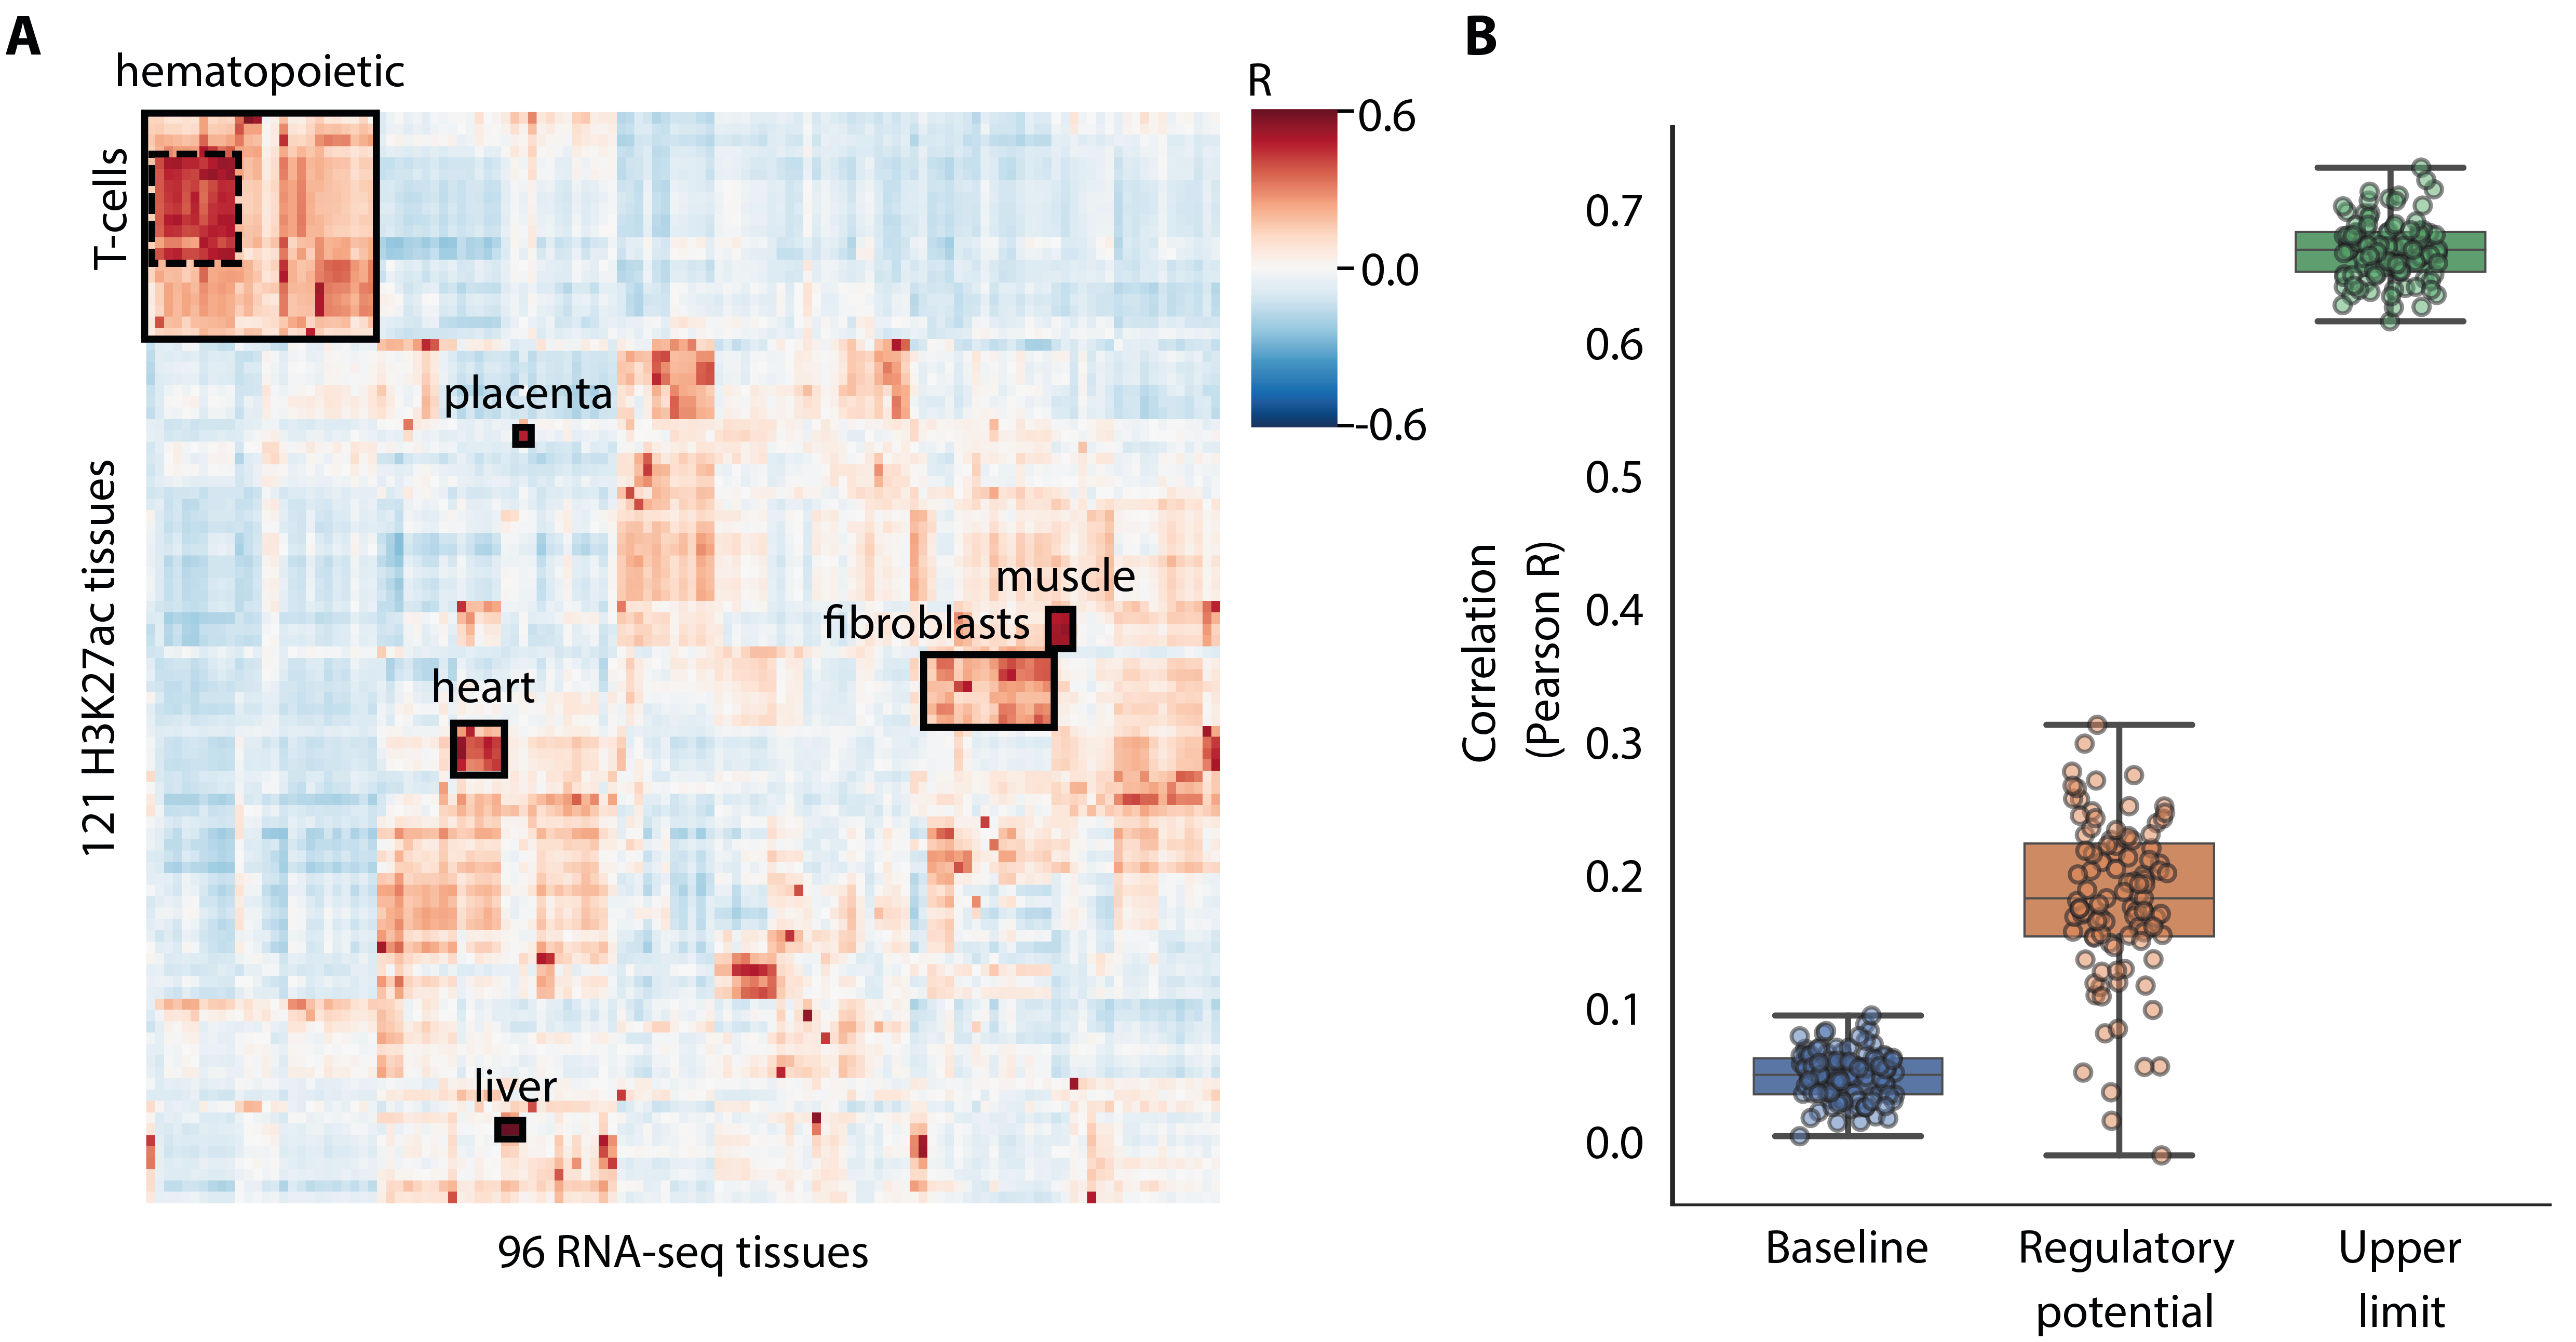
\includegraphics[width=1\linewidth]{ch.scepia/imgs/CellTypes_MvS_Myriad_Figure1.png}
    \caption{\textbf{Automatically matching epigenomic information to transcriptomic data improves motif activity inference.} \textbf{(A)}: The Pearson correlation coefficients between all combinations of regulatory potential of 121 H3K27ac cell types and TPM values of 96 RNA cell types. Rows and columns are hierarchically sorted, which clusters similar cell types in proximity, for example, the hematopoietic, heart, and muscle cells. \textbf{(B)}: Regulatory potential-based motif activities are superior to the baseline based on transcriptomic data alone. The motif activities of 5 random cell types are inferred based on the H3K27ac signal in the top 25,000 differential enhancers (100 permutations). The baseline approach to motif activity inference with only transcriptomic data is to assume that the TPMs of transcription factors are identical to their motif activity (mean correlation of 0.04). The regulatory potential-based approach automatically matches transcriptomic samples to H3K27ac samples in a hold-out set. It infers the motif activity scores on their top 10,000 differential enhancers (mean correlation of 0.17). Finally,  the upper limit evaluates the effect of the size of the enhancer set, and compares the inferred motif activities between enhancer sets the size of 10,000 and 25,000 (mean correlation of 0.66).}
    \label{fig:bulk_comparison}
\end{figure}

In general, the H3K27ac signal in regulatory sequences can be used to determine motif or transcription factor activity\cite{FANTOM2009,Balwierz2014,Madsen_2017}. This motif activity, which quantifies the contribution of each motif to H3K27ac peak strength, is a powerful measure of the relevance of a transcription factor for a specific cell state. The relationship between RNA-seq and regulatory potential led us to assume that transcription factor motif activity can be inferred from transcriptomic data, through an intermediate collection of matched H3K27ac data. As the reference collection contains a limited number of cell types, an exact matching cell type may not always be available for a specific cell type measured by RNA-seq. Therefore, we decided to calculate a composite measure of motif activity, based on a combination of reference cell types (see Methods). To calculate this measure, we regressed the TPM values of the 2,000 most variable genes of a collection of cell types against our regulatory potential database. From there, we selected the top 50 cell types based on the absolute regression coefficients and identified the top 10,000 most differentially enriched cis-regulatory regions within these 50 cell types. Subsequently, we calculated the motif activity using these enhancers and obtained the final motif scores by taking the dot product of motif scores and regression coefficients. 

To test the accuracy of this method, we made one hundred random subsets of five tissues common to both our H3K27ac reference database and transcriptomic dataset. Our first step involved establishing a ground truth for motif activities by conducting a motif scan on the top 25,000 most differentially enriched cis-regulatory regions within each of these five tissues. Here, these regions were defined based on a union of all public transcription factor binding peaks, as obtained from the ReMap database\cite{Chneby2017} (see Methods). As a baseline approach to estimating motif activity based solely on transcriptomic data, we assumed a direct one-to-one translation between the transcripts per million (TPM) values of a transcription factor and its motif score. However, as Figure \ref{fig:bulk_comparison}B illustrates, this baseline approach displays a particularly poor correlation with our ground truth (mean correlation of 0.04). Instead, our approach based on regulatory potential demonstrates a significantly improved correlation (mean correlation of 0.17). It is important to note that the cell types used for the ground truth are excluded from the reference database. Finally, to assess the sensitivity of our approach to the choice of cis-regulatory region set, we compared the ground truth data based on the top 25,000 most variable regions with that based on the top 10,000 most variable regions. Taken together, these analyses show that RNA-seq can be reliably matched to H3K27ac in a cell type-specific manner and that this data can be used to estimate transcription factor activity in a more reliable manner than gene expression alone. See supplemental figure \ref{fig:bulkbenchmark} for a one-factor-at-a-time parameter sweep, which shows that the results of SCEPIA are robust across a wide range of settings.

\subsection{SCEPIA accurately annotates single-cell populations and identifies known cardiac regulators}

We showed the possibility of matching cell type-specific H3K27ac-inferred regulatory potential to an RNA-seq dataset. SCEPIA was set up to incorporate this principle into single-cell transcriptomic analysis. Figure \ref{fig:scepia_overview}) shows a schematic overview of SCEPIA and individual step are explained in more detail in the Methods. In short, [...].  To evaluate performance, we conducted a comparative analysis on a multimodal dataset from the human Heart Cell Atlas v2 (hHCA; \cite{Kanemaru2023},) which encompasses over 700,000 cells profile scRNA-seq and spans the different anatomical regions and cellular subtypes of the human heart. We ran SCEPIA on the single cell transcriptomic assay of this atlas and used various strategies to evaluate the different steps incorporated in SCEPIA (Fig. \ref{fig:scepia_overview}). First, we ran SCEPIA on all cells of the atlas to asses its overall performance. We checked the intermediate outcomes of the run, such as the ability to annotate the cell type of the single cells correctly with the H3K27ac reference (Step 1 \& Step 2), as well as the inference of regulatory factors of importance (Step 3-5). 

\begin{figure}
    \centering
    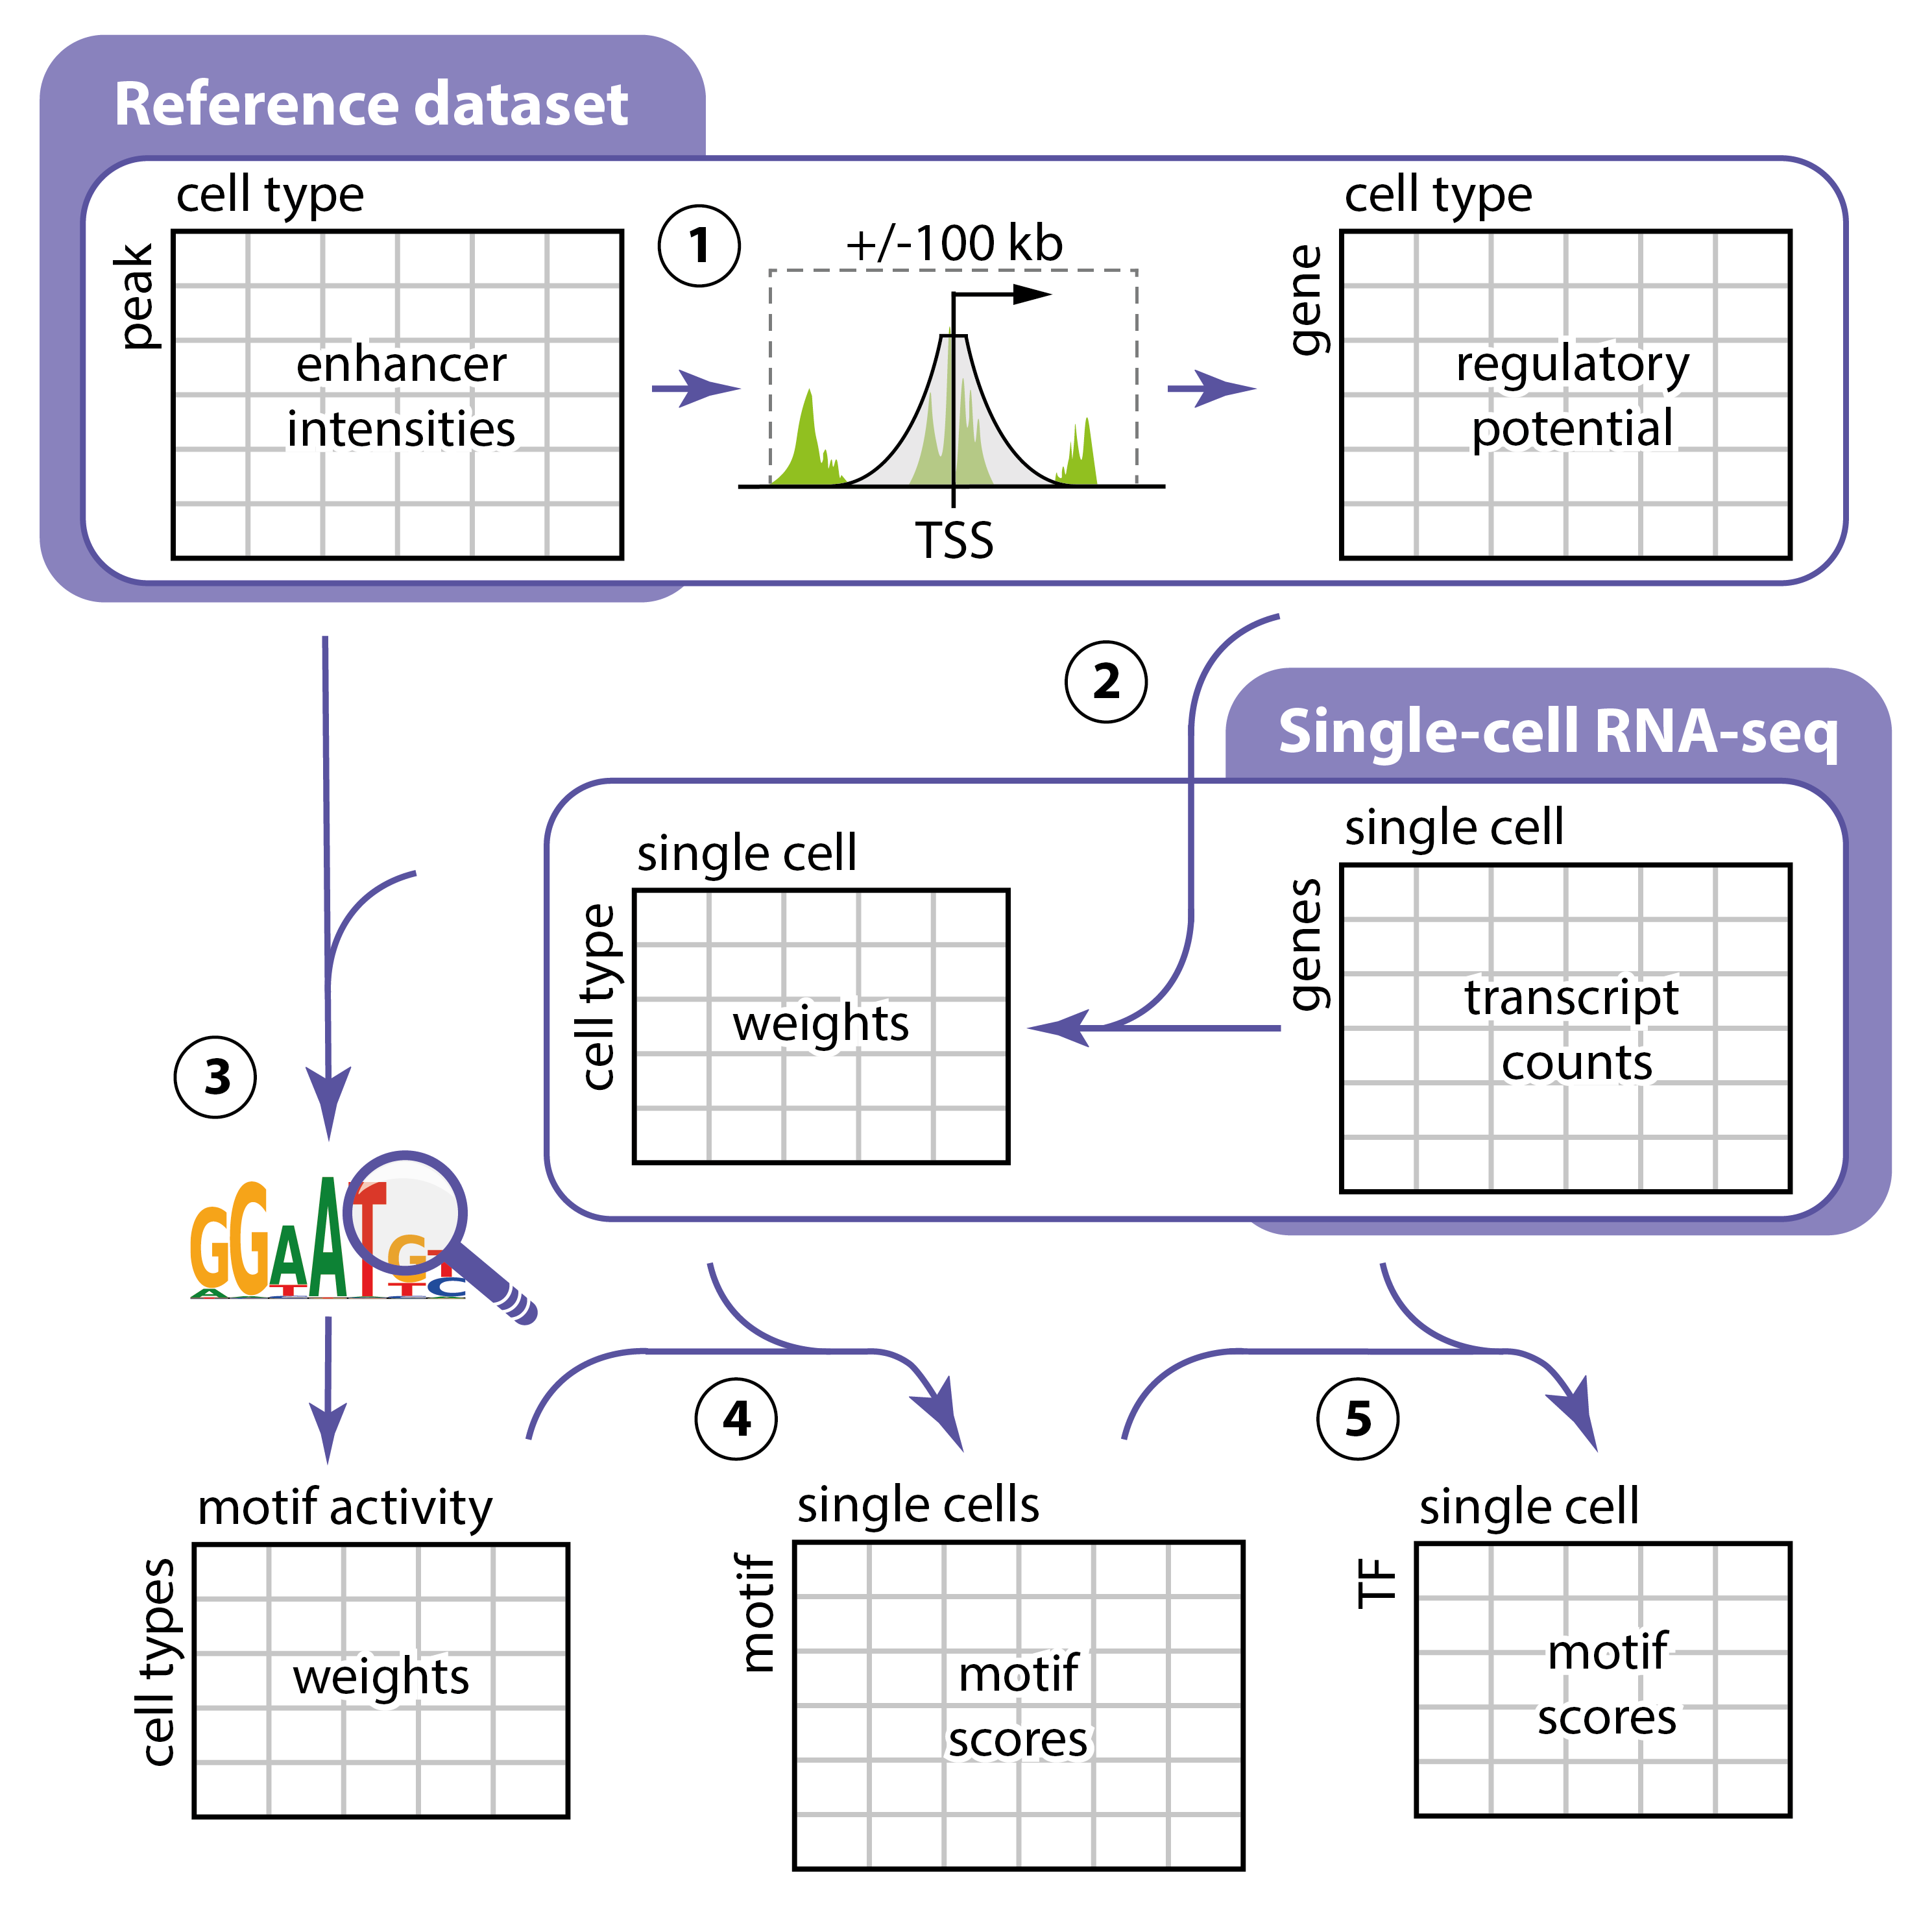
\includegraphics[width=1\linewidth]{ch.scepia/imgs/OverviewFigure_SvH_Myriad_v6_Figure2.png}
    \caption{\textbf{Overview of Single-Cell EPigenome-based Inference of Activity (SCEPIA).} See the methods for an extensive explanation per step. \newline 
    \textbf{Step 1}: Calculate the regulatory potential from distance-weighted chromatin assay intensities around each gene for each cell type in the reference collection.
    \textbf{Step 2}: Regress the single-cell gene expression on the regulatory potential. Keep the top 50 cell types with the absolute highest regression coefficients to use as the cell type weights for each cell.
    \textbf{Step 3}: Select the top 10,000 most differential \textbf{peaks/enhancers/...} between the top 50 cell types, and use them for motif activity inference.
    \textbf{Step 4}: Take the dot product between the motif activities and the cell type weights, resulting in motif activities for each motif per cell. Motif activities are scaled to a motif score between 0-1. 
    \textbf{Step 5}: Calculate the correlation coefficient between the expression level (log2 TPM) and the motif activity for TF-motif pairs. A permutation test between gene expression and motif activities allows for the estimation of the statistical significance of their relation.}
    \label{fig:scepia_overview}
\end{figure}

Accurate annotation of cell types by SCEPIA is important (Fig. \ref{fig:scepia_overview}: Step 2), as all subsequent analyses rely on this initial step. We demonstrated that this matching is accurate for bulk RNA-seq data (Fig. \ref{fig:bulk_comparison}A). To validate if matching of the reference also works on single-cell data, we compared the inferred annotation of SCEPIA (Figure \ref{fig:scepia_hhca1}A) with the cluster annotation as provided by the HCA authors (Figure \ref{fig:scepia_annotation1}A). SCEPIA correctly assigned the atrial and ventricular cardiomyocyte clusters to heart ventricle and cardiac atrium, respectively. The fibroblasts, neural cells and mural cells (i.e. smooth muscle cells or pericytes of the vasculature), all matched to tissues or cell types similar to their identity, albeit originating from a different organ or tissue (i.e. lung or tibia) (Figure \ref{fig:scepia_hhca1}A). Similarly, the myeloid and lymphoid clusters were matched with cell types from the correct major immune lineage branches, namely CD14+ monocytes and CD8+ T cells, respectively. SCEPIA had more difficulty annotating the endothelial cells, which showed the best match with heart left ventricle and a comparatively weaker match to umbilical vein endothelial cells (Fig. \ref{fig:scepia_annotation1}B). This may be attributed to the high prevalence of endothelial cells in the heart myocardium, as also evident from the cluster size of the endothelial cells in the atlas. Ultimately, in the analysis by SCEPIA, the endothelial cluster was represented by a combined signature of heart left ventricle and an endothelial cell type. Likewise, the adipocytes are represented by a mixed signature of right cardiac atrium and adipose tissue (Figure \ref{fig:scepia_annotation1}B). For the mesothelial cluster, there was no matching cell or tissue type available in the ENCODE database, which could explain the lack of any strong matches for this cluster. Overall, these findings highlight that SCEPIA matched the majority of the clusters correctly to the ENCODE reference. 

Following the initial annotation of cell types, we investigated the transcriptional regulators considered important by SCEPIA in these clusters. Among the top 15 hits, as ranked by correlation coefficient, were several known markers for various cell types present in the atlas (Figure \ref{fig:scepia_hhca1}B). Examples include \textit{FLI1}, \textit{ETS1} and \textit{KLF2} for immune and endothelial cells \cite{Meadows2009,Zhao2018,BenDavid2022}, \textit{TBX5} for cardiomyocytes\cite{Steimle2017,Siatra2023}, \textit{HEY1} for atrial cardiomyocytes \cite{Kokubo2007}, and \textit{PPARG} for adipocytes \cite{Ma2018}. SCEPIA correctly predicted the motif activity of \textit{TBX5} in the cardiomyocyte clusters, which also aligned with its expression pattern (Figure \ref{fig:scepia_hhca1}C). Predicted motifs for \textit{SOX17} and \textit{RUNX1} exhibited variable motif activities, with expected higher activities in endothelial and lymphoid clusters, respectively (Figure \ref{fig:scepia_hhca1}C)\cite{Lee2014,Schachterle2017,Sood2017}. \textit{BACH2} is a known repressor and immune-regulating transcription factor and is also implicated in neural differentiation\cite{Hoshino2002,Liu2022}. \textit{BACH2} is most highly expressed in neural and lymphoid cells, where the motif activity (bZIP.0003) was decreased, and reason for SCEPIA to identify this TF as a repressor (Figure \ref{fig:scepia_features1}A). However, the inferred motif activity of \textit{BACH2} was increased in the myeloid and endothelial cluster, contradicting its established role as repressor in myeloid cells. \textit{BACH2} is known for its repressive regulatory functions in myeloid lineages \cite{ItohNakadai2014}, and was recently described for its activator role in B-lymphocytes\cite{Ochiai2022}. This duality, seemed to pose a challenge for  correct inference of the activity for this factor in these cell types. This could be attributed to the absence of particular cellular subtypes in the H3K27ac reference, restricting the full capture of \textit{BACH2}'s complex  transcriptional regulation in immune populations. To further confirm the regulatory role of \textit{BACH2} in this dataset, we checked the expression level for putative target genes, based on ChIP-seq (Fig. \ref{fig:scepia_features1}B). The compound expression level of 57 predicted \textit{BACH2} targets, showed patterns of expression reminiscent to the motif activity as predicted by SCEPIA, and thereby for many clusters, the reversed of \textit{BACH2} expression itself. These findings indicated that openness of the motif is indeed correlated with the activation of target genes nearby, and in clusters with increased \textit{BACH2} expression, the openness of the motif decreases. These findings underscore the difficulty of distinguishing some of the more complex regulatory roles of TFs. However, altogether SCEPIA mostly identified relevant regulators, as well as a well-known repressive regulator.

\begin{figure}
    \centering
    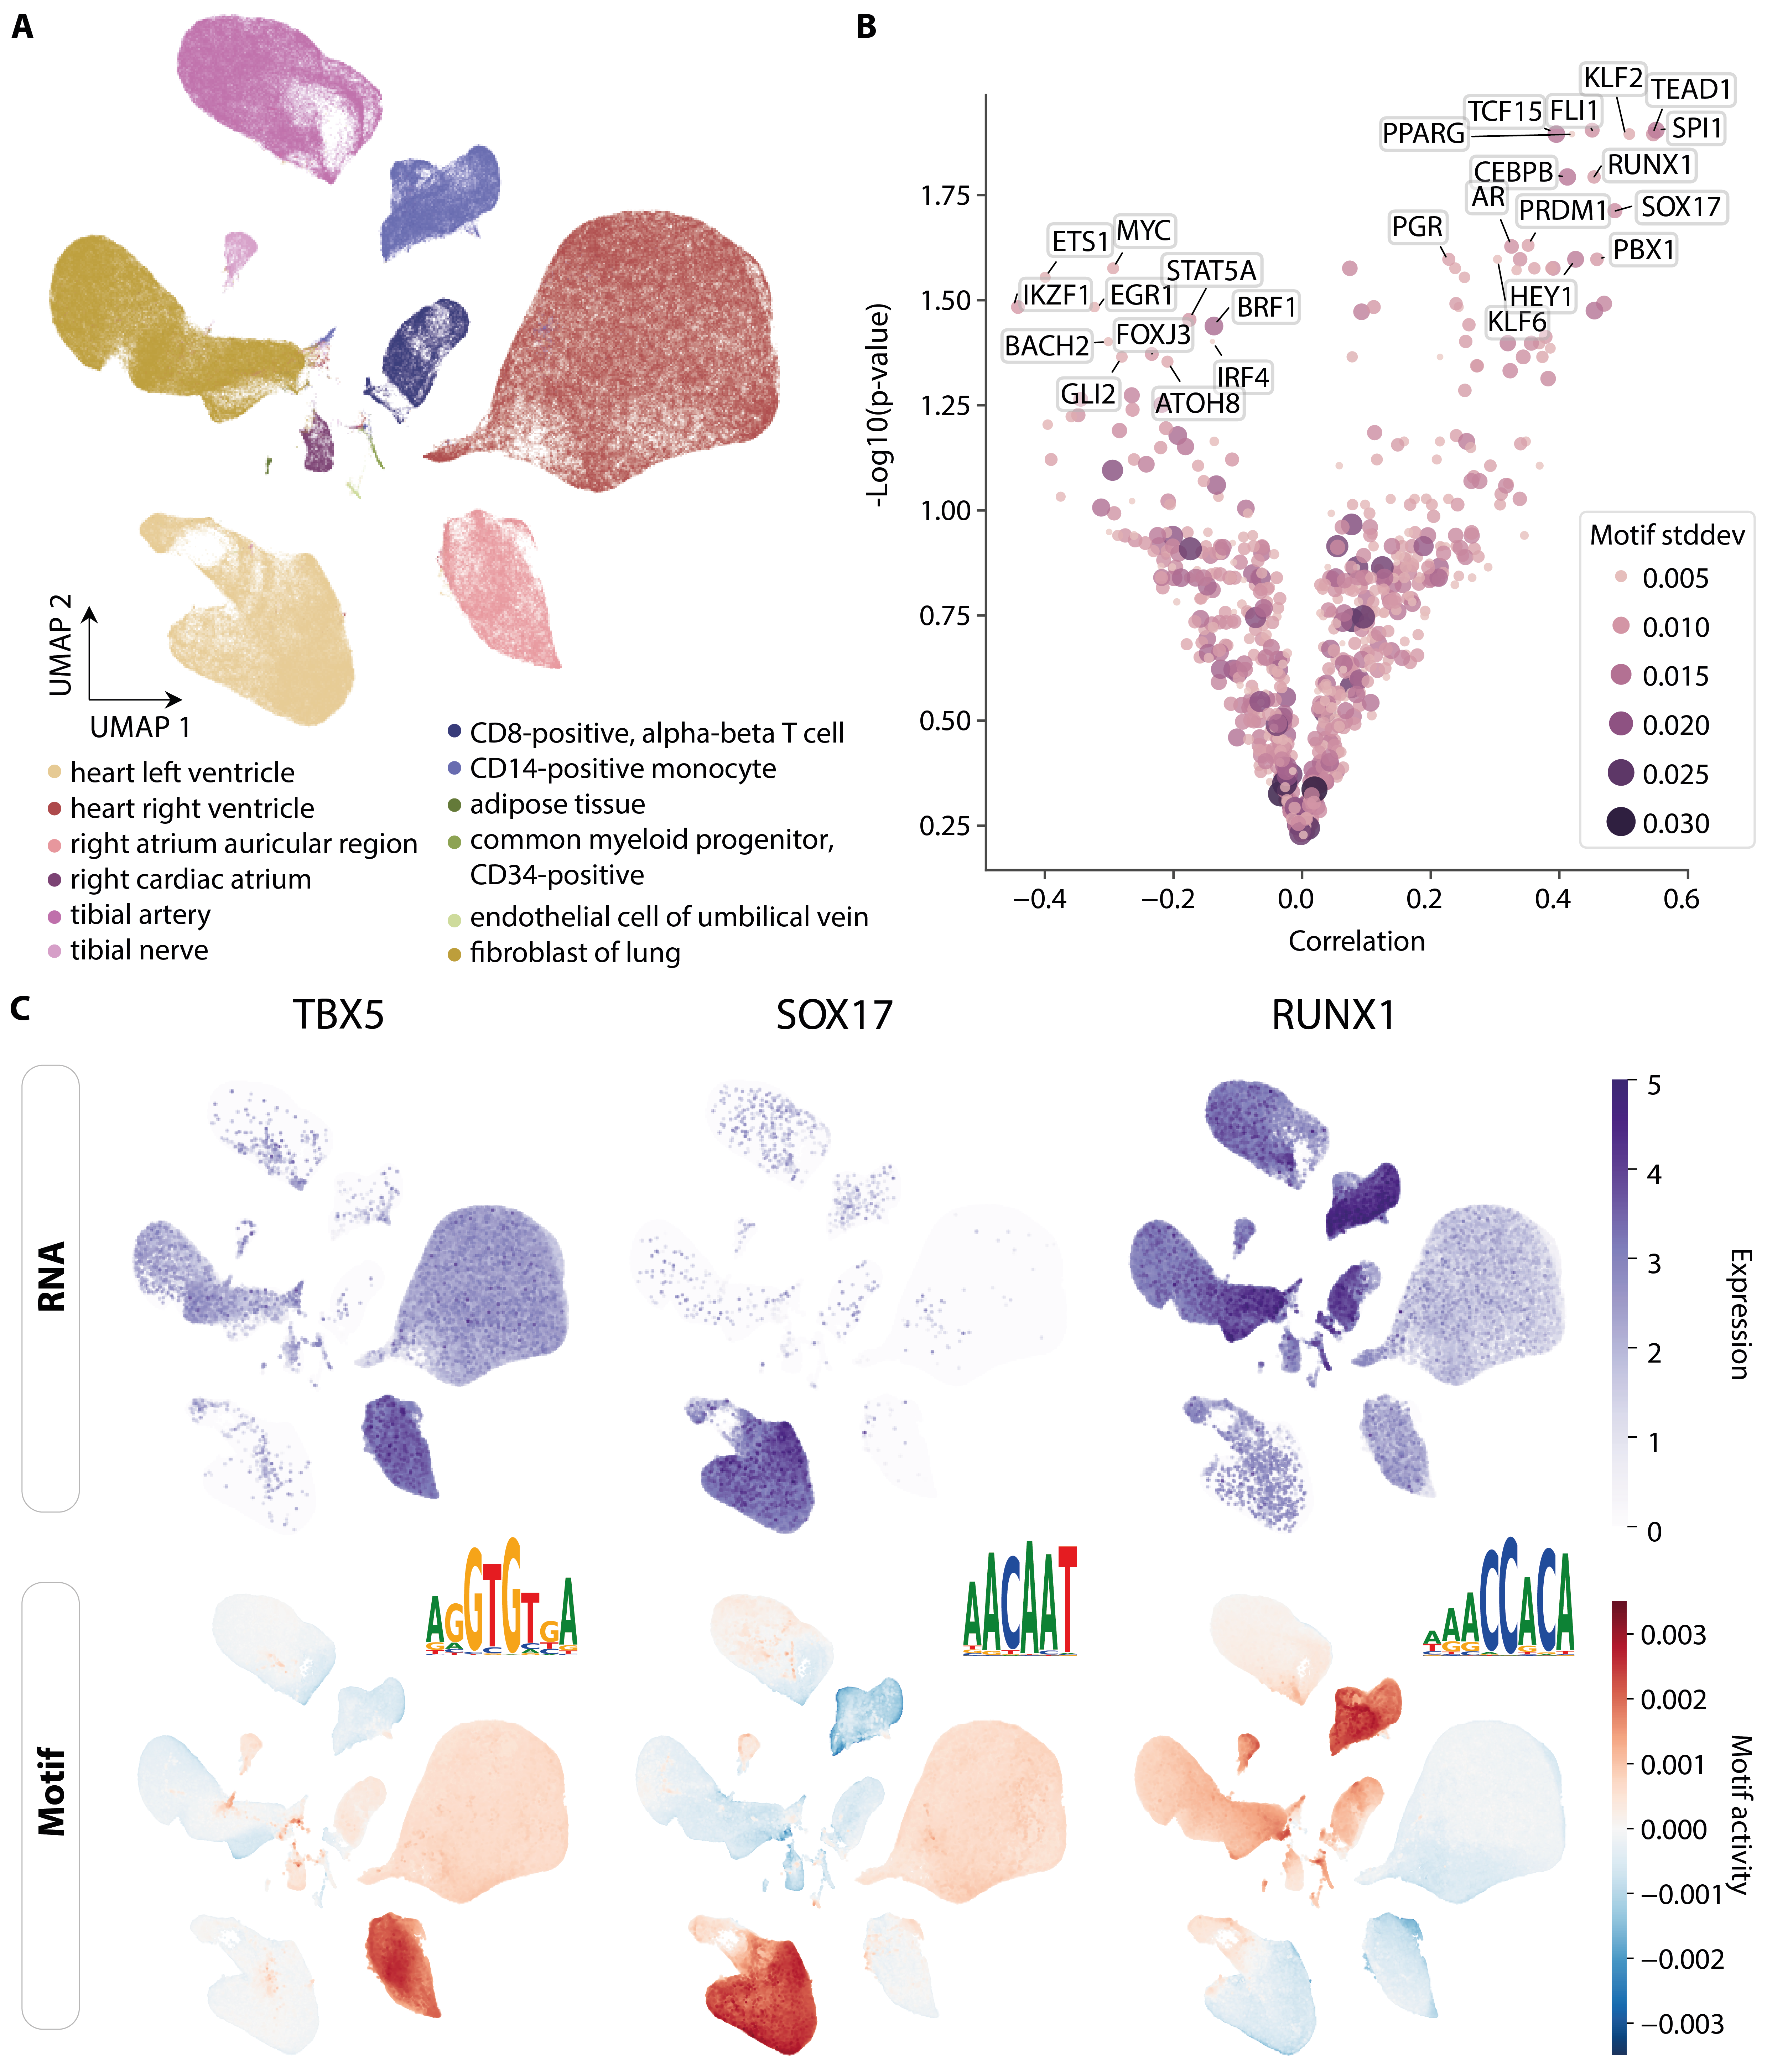
\includegraphics[width=0.75\linewidth]{ch.scepia/imgs/SCEPIA_allCells_v10_Myriad_Figure3.png}
    \caption{\textbf{Transcription factor activity in Human Heart Cell Atlas predicted by SCEPUA} \textbf{(A)} UMAP representation of all cells in the hHCA, based on UMAP coordinates provided by the original study\cite{Kanemaru2023}, with cluster annotation labels as predicted by SCEPIA. \textbf{(B) }Volcano plot of SCEPIA hits, [explain X an Y]. The top 15 transcription factors are labeled, for putative posituve regulators as well as putative repressers. [... explain p-value in somehwat more detail..]s. Dot size and color labels are based on the motif score standard deviations.  \textbf{(C) }Expression level (top) and the predicted motif activity by SCEPIA (bottom),of three well-known markers: TBX5 (cardiomyocytes), SOX17 (endothelial cells), RUNX1 (blood cells). Visualization is based on the UMAP coordinates as shown in A. Sequence logos of the binding motifs are indicated, with the GimmeMotifs database identifiers (left to right): GM.5.0.T-box.0005, GM.5.0.Sox.0021, GM.5.0.Runt.0003. }
    \label{fig:scepia_hhca1}
\end{figure}


\subsection{Prioritization of cardiac regulators by SCEPIA improves with directed subsampling of abundant cell types}

For a subset of the hHCA, chromatin accessibility data (scATAC-seq) is available. For this data set, the chromatin accessibiity was measured in the same nucleus as the transcriptomic data. This offered an ideal use-case for benchmarking SCEPIA. The multimodality allows for a comprehensive evaluation of transcriptional regulators identified by SCEPIA, as the predicted motif activity can be compared to the motif activity based on the scATAC-seq data. First, we ran motif analysis on the pseudobulk of the scATAC-seq clusters using GimmeMotifs Maelstrom\cite{Bruse_2018} (hereafter referred to as maelstrom analysis), to infer the cell type-specific motif activities. As mentioned, SCEPIA is tailored to infer enhancer activity from H3K27ac reference data. Although, the information on chromatin context between H3K27ac and ATAC-seq differs (active enhancers versus accessibility of chromatin, respectively), the motif analysis on the pseudobulk ATAC-seq served in this case as our closest approximation to a ground truth. 

To establish a baseline of correlation coefficients for our further comparisons, we compared the TF expression levels with their binding-motif activities in the measured accessible chromatin within the hHCA. This was considered our baseline comparison since it was performed without any prioritization between motif-TF links, and solely based on the predicted motif-TF links from the GimmeMotifs database. To enable multiple runs in our comparisons and evaluate reproducibility, we divided the scRNA-seq data into seven random subsets, each consisting of 100K cells. Next, we correlated the motif activities computed with the maelstrom analysis with the expression levels of each TF binder across the cell types, and for each subset. This comparison yielded coefficients ranging from a r of -0.02 to 0.26 (Fig. \ref{fig:sc_benchmark} blue) and reflected the degree of similarity between TF expression levels and their motif activities measured in a single-cell multi-modal setting.

To benchmark SCEPIA against these results, we compared the SCEPIA runs on each of these seven subsets to the maelstrom analysis. For all the significant SCEPIA hits (p-adj < 0.05), we averaged their inferred motif activities per cell type. These averages were correlated to the activities for the same motifs from the maelstrom analysis. Interestingly, the mean coefficients per cell type in these correlations were consistently higher than those found in the baseline comparison, except for the mesothelial and mural cell cluster (Fig. \ref{fig:sc_benchmark} orange, Table \ref{tab:significance_scbenchmark}). However, these scores exhibited substantial differences across the cell types, with a median r ranging from 0.14 for the mesothelial to 0.58 for the myeloid cluster (Table \ref{tab:significance_scbenchmark}).

As we observed variations in the performance across the cell types, with some scoring lower (e.g. cardiomyocyte clusters, fibroblasts and endothelial cells, with a median r < 0.4), than others (myeloid and mast cell clusters, median r > 0.4), we implemented a step of geometric sketching. Geometric sketching is a method that subsamples the cells in the dataset while preserving the inherent heterogeneity, or geometry, of the dataset \cite{Hie2019}. Since a geometric sketch will lead to a more equal representation of the different cell types across the dataset, including rare cell types, we included this subsampling step during the pre-processing of the data and preceding the SCEPIA run on each of the seven subsets (see Methods). This significantly improved the correlation coefficients with the maelstrom results for both cardiomyocyte and endothelial clusters, as well as the myeloid cluster (Fig. \ref{fig:sc_benchmark} green, Table \ref{tab:significance_scbenchmark}). The neural and adipocyte, mural and mesothelial cell-clusters displayed more variability in their coefficients, with some obtaining equal or worse coefficients after the addition of the geosketching. While the geometric sketch could not fully alleviate the low performance of SCEPIA for certain cell types, incorporating this step significantly improved the performance for five out of the twelve cell clusters in this specific benchmark. 

\begin{figure}
    \centering
    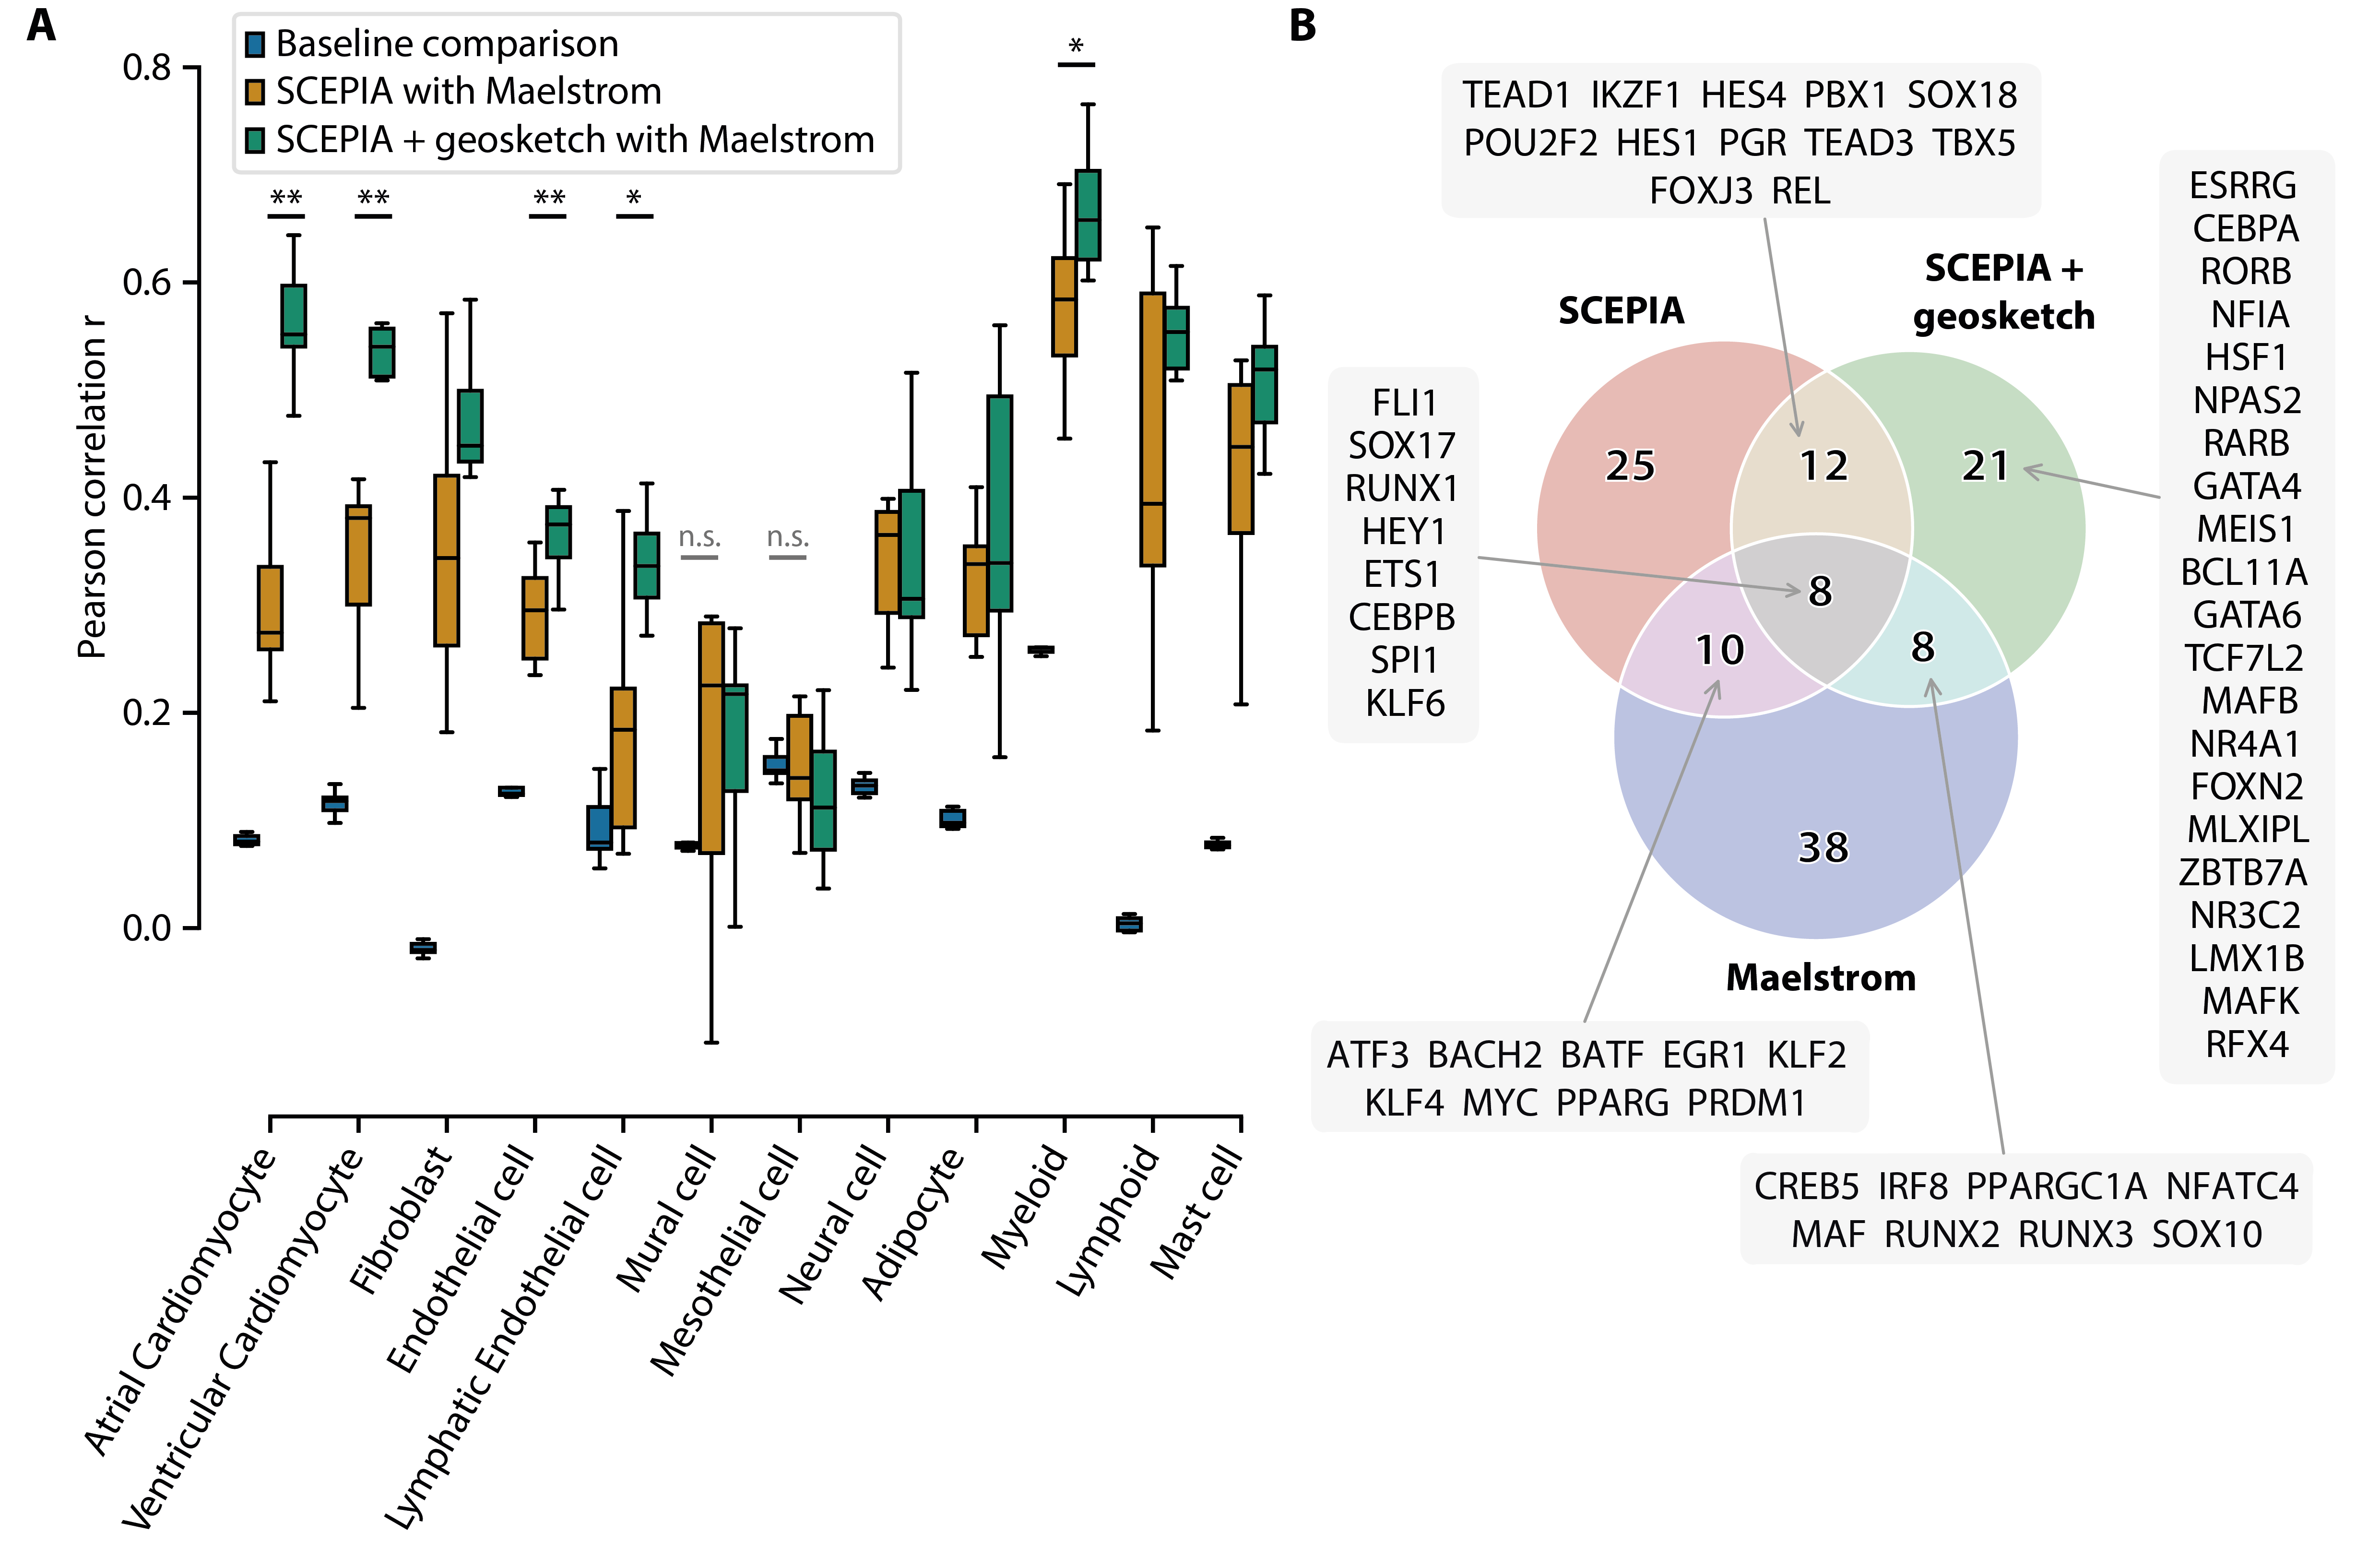
\includegraphics[width=0.75\linewidth]{ch.scepia/imgs/OverlappingHitsBetweenSCEPIAGEOANDMAELSTROM_BlackMyriad_onlySign_baselineNS_v11_Figure4.png}
    \caption{\textbf{Benchmarking SCEPIA} (\textbf{A}) Correlations between motif activity computed in pseudobulk ATAC-seq fraction (maelstrom analysis) and expression values of their TF binders from each of the seven 100K cells scRNA-seq subsets (blue; Baseline correlations). In orange the motif activities of significant (p-adjusted < 0.05) SCEPIA hits from each of the seven 100K subset analyses, were correlated with the matched motif activities computed with the maelstrom analysis (SCEPIA with Maelstrom). Green represents the correlation coefficients of the comparisons with maelstrom motif activities, for the seven 100K subset runs with SCEPIA with prior pre-processing with geometrical sketch subsampling of each of the seven 100K cells subsets (SCEPIA+geosketch with Maelstrom). Significance of differences between conditions calculated with one-sided Wilcoxon signed-rank test. Only non-significant results are indicated for the baseline versus SCEPIA comparison in grey, and only significant results indicated for the SCEPIA versus SCEPIA+geosketch comparisons (all p-values can be found in Table \ref{tab:significance_scbenchmark}).  **: p-value <= 0.01, *: p-value <= 0.05, n.s.: non-significant. (\textbf{B}) Venn diagram presenting overlaps and differences between the SCEPIA runs on the full dataset (700K cells of the hHCA), the SCEPIA run with geosketch subsampling of the full dataset (subsampling 700K to 20K cells) and the maelstrom analysis on the pseudobulk of the scATAC-seq data of the hHCA. hHCA = human Heart Cell Atlas.}
    \label{fig:sc_benchmark}
\end{figure}

\subsection{SCEPIA Identifies Additional Cardiac Regulators Compared to Motif Analysis in ATAC-seq} 

To validate our approach in selecting regulatory factors based on motif activity and TF expression patterns, we compared the outcomes of SCEPIA with a selection based on motif activity alone. Given the improved performance of SCEPIA across various cell types with the inclusion of a step of geosketching, we further examined its efficacy by downsizing the full dataset to a geosketch of 20K cells and reran SCEPIA (Fig. \ref{fig:geoscepia_results}). We then explored biological differences between the methods.

Of the 49 total hits, the geosketched SCEPIA run yielded 20 overlapping hits with the full dataset run and a partial overlap with TFs linked to maelstrom motif hits (16 hits; Figure \ref{fig:sc_benchmark}B). Common hits, such as \textit{FLI1} and \textit{SOX17}, implicated in cardiac cells, as well as \textit{HEY1} (cardiac progenitor marker) and \textit{ETS1} (lymphoid marker), reaffirmed SCEPIAs consistency. The maelstrom analysis pointed to variable motif activity for a BACH2-binding motif and indicated higher activity in the fibroblast, endothelial and mesothelial clusters. The first SCEPIA run inferred increased motif activity for \textit{BACH2} in these same clusters, with additional high levels in the myeloid and mural cells (Figure \ref{fig:scepia_features1}A). However,  differences also emerged between the runs. \textit{GATA4} and \textit{GATA6} for example, vital for cardiac (mesoderm) development and inferred with increased motif activities in the cardiomyocyte clusters, were exclusively found in the run on the data preprocessed with geosketch (Figure \ref{fig:scepia_features1}C) \cite{Morrisey1996,Song2022}. Notably, \textit{GATA1} was only identified in the non-geosketched run, showing specific expression and increased motif activity in mast cells (Figure \ref{fig:scepia_features1}D), a cell type-specificity confirmed in literature \cite{Migliaccio2003,Gao2015}. \textit{RUNX1} was consistent, while \textit{RUNX2} and \textit{RUNX3} were additionally identified in the geosketch run, all linked by SCEPIA to the same motif (Runt.0003). The motif activity changed to be more restricted to immune cells in the geosketch run, whilst in the run without geosketch this motif activity was additionally inferred across, for instance, the mural, neural and fibroblast cells (Figure \ref{fig:scepia_features1}E, \ref{fig:scepia_hhca1}C).

Some specific overlaps of interest were seen between the geosketch SCEPIA run and maelstrom analysis. Regarding the \textit{SOX} gene family, \textit{SOX17} and \textit{SOX18} were already identified in the first SCEPIA run, coupled to motifs with similar activities over the clusters. The SCEPIA run on the geosketched dataset additionally inferred \textit{SOX10} in the neural cluster and to a lesser degree in the endothelial cells (Figure \ref{fig:scepia_annotation1}F). Similarily, in the maelstrom analysis, two \textit{SOX10} motifs ranked among the top three highest-scoring motifs in the neural cluster (Sox.0018 and Sox.007; Figure \ref{fig:scepia_maelstromhm}). Maelstrom inferred the fibroblast cluster as the second highest in terms of motif activities in one case, and the endothelial cluster for the other. Furthermore, SCEPIA identified next to a similar specificity of motif activity for \textit{SOX10} (Sox.0034; Figure \ref{fig:scepia_features1}F), also a sequence motif that was similar, i.e. a subset, of the motifs inferred by maelstrom (Figure \ref{fig:scepia_features1}G). Differences included \textit{IKZF1}, identified by SCEPIA with an inferred activity in almost all clusters, with only a specific depletion of signal in the immune clusters (Fig. \ref{fig:scepia_features2}B, D), aligning with its dual repressor and activator role in immune cells \cite{Marke2018}. Other examples include, \textit{TBX5} and \textit{MEIS1}, both well-known cardiac mesoderm markers, alongside \textit{ESRRG}. Some of the binding motifs for these factors were inferred to have a certain level of activity across multiple clusters in the dataset, and only by considering the expression levels of these factors, a specificity could be distinguished (example of \textit{ESRRG} in Fig. \ref{fig:scepia_features2}A, C). Conversely, there were also hits in Maelstrom, that were not identified in any of the SCEPIA runs. A notable discrepancy involved the \textit{MEF2} transcription factor family..Maelstrom analysis showed motif enrichment in cardiomyocytes and mural cell clusters, however, the expression levels of \textit{MEF2A-D} were consistent across the majority of cell types (Fig. \ref{fig:scepia_features2}E) and showed low correlations with their inferred motif activities (Tables \cite{tab:corrtable_SCEPIA,tab:corrtable_GeoSCEPIA}), which could explain the absence in SCEPIAs hits. These findings suggest that SCEPIA is better suited in identifying factors with ubiquitous motif activities, because of the inclusion of expression level information in selecting the factors. Conversely, if the expression of the factor is not highly variable or not well (anti-)correlated with the predicted motif activities, SCEPIA will overlook these factors, even if the binding motifs were inferred with variable activities over the cell types.

\section{Discussion}

In this study, we present SCEPIA, a novel computational method for inferring transcription factor motif activities using single-cell transcriptomic data in combination with a reference H3K27ac collection. SCEPIA successfully identifies established key regulators in various cardiac cell types, including endothelial cells (\textit{FLI1}), cardiomyocytes (\textit{TBX5}, \textit{HEY1}), adipocytes (\textit{PPARG}), and immune cells (\textit{RUNX1}), in addition to recognizing the suppressor \textit{BACH2}. This method stands out by leveraging pre-existing bulk epigenomic data, thus augmenting single-cell transcriptomics datasets and creating a multimodal resource for the identification of transcription regulators.

SCEPIA matches cells to a combination of known H3K27ac signatures, thereby establishing new H3K27ac identities that are not explicitly defined in the reference. In the case of endothelial cells and adipocytes, which were both missing from the reference, this approach has demonstrated that it can identify appropriate key TFs (\textit{e.g.} \textit{FLI1} and \textit{PPARG}). However, we faced challenges with the identification of key TFs for other cell types that were not in the reference, such as mesothelial or mural cells. This difficulty likely arises from two main issues: the lack of closely related cell types in the reference dataset (for example, epicardial cells) and the low number of these cells in the cardiac tissue samples we studied. One solution for this could be found in applying another epigenomic assay or expanding on the current ChIP-seq reference in SCEPIA. SCEPIA already includes pre-built alternative references from diverse sources, such as scATAC-seq datasets of fetal human cell types\cite{Domcke2020} and various adult mouse tissues\cite{Cusanovich2018}. Expanding the provided references with other epigenomic collections, either generated by the researcher themselves or using readily available and vast collections (e.g. SRA) could greatly enrich SCEPIA's reference database and potentially improve its accuracy and applicability, also for more rare subtypes. 

The transcription factor \textit{MEF2C} plays a crucial role in chromatin remodeling which increases DNA accessibility in cardiomyocytes\cite{Stone2019,Ieda2010,Desjardins2016} and during neural development\cite{Li2008}. Despite its important role, SCEPIA did not identify \textit{MEF2C} or other members of the \textit{MEF2} family, as key cardiac regulators. Whereas, in our comparison based on single-cell DNA accessibility alone, their motif was flagged for its differential inferred activity. Even though we observed a variable gene expression of \textit{MEF2C} across different cell types, there was a poor match between the gene expression levels and predicted motif activity. This exemplifies the complex nature of \textit{MEF2C}'s role in regulating genes during heart development. \textit{MEF2C} is known to produce several isoforms that regulate different genes\cite{Zhu2004}. Additionally, \textit{MEF2} factors often form hetero- or homodimers to more precisely regulate their target genes \cite{Desjardins2016,Black1998}. The complexity of the \textit{MEF2} gene regulatory function demonstrates the drawback of transcriptomic-based regulator inference methods, including SCEPIA. These methods cannot account for post-transcriptional modifications, and as such cannot fully capture the regulatory roles of transcription factors like for instance, \textit{MEF2C}.

Establishing an accurate baseline and ground truth presents a significant challenge in our study, particularly when it comes to benchmarking the results of SCEPIA. For the single-cell comparisons, our ground truth is calculated on regression coefficients based on a measure of DNA accessibility. However, SCEPIA uses a different reference, based on H3K27ac, a marker for active cis-regulatory regions. Whilst DNA accessibility and H3K27ac generally coincide, these two assays measure distinct aspects of chromatin context and gene regulation. For instance, our SCEPIA analysis identified nuclear receptor motifs, such as \textit{TBX5} and \textit{GATA4}, using the H3K27ac reference. These motifs were not detected based on our analysis of scATAC-seq data. This discrepancy can be attributed to the nature of these transcription factors: \textit{TBX5} and \textit{GATA4} need co-factors to bind the chromatin and activate their targets, and are not able to bind previously inaccessible regions\cite{Stone2019}. Therefore, ideally, both the reference database and the ground truth are based on the same assay. Additionally, the motif activities based on DNA accessibility in SCEPIA are inferred by the ensemble computational method GimmeMotifs Maelstrom\cite{Bruse_2018}. As a consequence, the ground truth of this study is based on a computational analysis rather than an experimentally validated ground truth. Taken together, the direct comparison of SCEPIA's benchmark results requires careful interpretation.

We foresee several ways to improve the current implementation of SCEPIA. First, is the appropriate selection of highly variable genes and relevant cells. Currently, SCEPIA selects the top 2,000 genes based on dispersion-normalized gene expression, which may inadvertently bias the analysis towards overrepresented cell types. Potentially more sophisticated approaches could be used, such as comparing the highly variable genes between clusters, performing geometry-preserving sampling (geosketch)\cite{Hie2019}, or selecting genes based on selectively detected or undetected expression in a particular cell neighbourhood (SEMITONES)\cite{Vlot2022}. Cell sampling methods that represent all distinct cell types, such as geosketch, have as an added benefit that the TF-motif significance calculation will be improved. Currently, TF-motif significance is calculated with a permutation test of the correlation between TF and motif. The presence of large groups of similar cells influence this calculation, therefore a more representative subsampling of the data could be beneficial. Second, SCEPIA could be improved by incorporating additional genomic assays. Given the similarities between H3K27ac and ATAC-seq data, integrating an extensive ATAC-seq collection seems promising. SCEPIA already includes pre-built references from diverse sources, such as scATAC-seq datasets of fetal human cell types\cite{Domcke2020} and various adult mouse tissues\cite{Cusanovich2018}. Third, is a refinement of the permutation test on the correlation coefficient between TF and motif activity. The relationship between TF gene expression and its motif activity is often unclear. Instead, a more informative relationship can be found between motif activity and the gene expression of downstream genes. Given that SCEPIA includes a comprehensive reference of cis-regulatory regions, these regions can be associated to their nearest gene, although this approach has its limitations\cite{Fulco_2019}. By establishing this association, we can link motif activities directly with specific genes, thereby basing the significance test on a more direct and relevant relationship. Moreover, combining these relationships with the expression of the TF itself, provides a clearer understanding of the functional impact of TFs within regulatory networks.

Single-cell omics datasets provide a detailed view of transcription regulation unique to each cell type, enabling the exploration of lesser-known and more challenging-to-obtain populations within tissues. Given that heart and vascular diseases are among the leading causes of death worldwide\cite{Tsao2023}, it is crucial to better understand epigenomic (dis)regulation at a cellular level. Our study introduces SCEPIA, a powerful computational tool designed to enrich transcriptomic data with transcription factor motif activity. This enhancement facilitates the precise identification of regulators specific to different cell types. SCEPIA's capability to integrate detailed transcription factor information into single-cell transcriptomics paves the way for a more comprehensive understanding of how transcription is regulated in various cell types.

% In this study, we present SCEPIA, a computational method for the inference of transcription factor motif activities based on single-cell transcriptomic data in combination with a reference H3K27ac collection. SCEPIA identifies known regulators for endothelial (\textit{FLI1}), cardiomyocyte (\textit{TBX5}, \textit{HEY1}), adipocyte (\textit{PPARG}) and immune (\textit{RUNX1}) cell types, as well as the known suppressor\textit{BACH2}. Additionally, we show that one can reliably match cell types based on transcriptomic abundances and H3K27ac-based regulatory potential\cite{Wang2016}, both in the case of bulk and single-cell RNA-seq. This means that SCEPIA leverages already existing bulk epigenomic data sources to expand on a single-cell transcriptomics dataset, thereby creating a single-cell multimodal resource for transcriptional regulator identification.


% A substantial amount of knowledge exists on marker genes and regulators in cardiac tissues, which allowed us to validate the accuracy of SCEPIA's hits. However, not all of rarer cell types within the heart have received this extensive attention. Therefore relying on a reference dataset has notable drawback—specific cell types, especially rare ones, may be absent—SCEPIA addresses this limitation by matching single cells to mixed signatures, establishing new identities not explicitly present in the original reference. This flexibility was shown advantageous for certain cell types, as demonstrated with endothelial cells and adipocytes. Nonetheless, matching of certain cell types, such as mesothelial or mural cells, remained difficult. This difficulty likely stemmed from the absence of any closely resembling cell type in the reference (e.g. epicardial cells), and potentially low abundances of this particular type in tissue samples. The same holds true for other rare populations in the cardiac tissues that are increasingly gaining interest in terms of their molecular mechanisms of regulation to for instance culture these cells \textit{in vitro}, like the pacemaker cells and nodal cells, but which we therefore did not focus on in the current study.


% difficult biological examples for SCEPIA
% Another complex regulatory example is \textit{MEF2C}, a factor that can promote chromatin remodeling at previously inaccessible sites and an activator of cardiomyocyte genes (\href{https://doi.org/10.1016/j.stem.2019.06.012}{https://doi.org/10.1016/j.stem.2019.06.012}, https://pubmed.ncbi.nlm.nih.gov/20691899/, https://www.ncbi.nlm.nih.gov/pmc/articles/PMC5019174/) and needed in neural development (https://pubmed.ncbi.nlm.nih.gov/18599437/). None of the \textit{MEF2}-family factors, were identified in the SCEPIA analysis, whereas their binding motifs were identified in the maelstrom analysis. \textit{MEF2C}, and other \textit{MEF2} factors, showed variable expression levels across the cells in the dataset, however, the correlations with its predicted motif activities were low (<0.XX INCLUDE CORRELATIONS TABLE OF SCEPIA IF NEEDED XX and add in results). The mechanisms of gene regulation by \textit{MEF2C} in cardiac development, are complex. The \textit{MEF2C} gene produces multiple isoforms, described to regulate different genes (https://www.ncbi.nlm.nih.gov/pmc/articles/PMC515034/), while generally the \textit{MEF2}-factors form different hetero- and homodimers to fine-tune its activator function in the regulation of their target genes (https://www.ncbi.nlm.nih.gov/pmc/articles/PMC5019174/, \href{https://doi.org/10.1146/annurev.cellbio.14.1.167}{https://doi.org/10.1146/annurev.cellbio.14.1.167} ). This illustrates the difficulties in correctly identifying this and other similarly complex TFs solely based on single-cell RNA-seq and motif activity read-outs, due to the challenges of accounting for the modifications of a TF after transcription, as well as the added complexity of the TFs' reciprocal influences on their transcriptional regulation. % A partial solution could be found in also analysing co-occurance of multiple motifs in cis-regulatory regions?


% scepia vs scenic
% The post-transcriptional and -translational modifications of TFs are challenging steps of regulation to infer without the direct measurement of protein levels. Our current implementation of SCEPIA infers the TF protein activity by taking along the motif activity, and subsequently generates a list of TF and motif combinations that are significantly correlated across the cells in the dataset. This approach has the advantage of also selecting factors that show correlating patterns of activity independent of cell cluster boundaries. A downside of this approach is, however, SCEPIA does not infer any gene regulatory networks and ignores any links between TFs and their target genes. Moreover, correlations between transcripts and their protein levels are particularly poor\cite{Fortelny2017,Franks2017}, and likewise, in some cases of confirmed cardiac regulators we find a low correlation between transcription factor mRNA levels and motif activity. This also occurs in cases where there is variability measured in one or both of the modalities (i.e. indicating a motif or TF of interest). In these cases correlations are unable to uncover the complex relationship between TF expression and the TF motif binding. An alternative way to prioritize factors, is to correlate the expression of target genes with the motif activity inferred nearby its promoter or enhancer regions. We assessed this for one example in our analysis, the repressor \textit{BACH2}. The expression of \textit{BACH2} target genes showed a similar pattern to the motif activity predicted by SCEPIA, which further highlights the potential regulatory role of this factor. Furthermore, a similar computational tool for identification of TF regulators in scRNA-seq, SCENIC\cite{Aibar_2017}, incorporates information on co-expression of TFs with target genes. The resulting gene regulatory networks are subsequently refined based on whether the DNA-binding motifs of TFs are present in the cis-regulatory regions of the co-expressed target genes. Augmenting SCEPIA to infer co-expression-based networks would allow for the combination of SCEPIA's refined way to incorporate detailed cell type-specific epigenomic signals, with SCENIC's ability to incorporate target gene information, and a gene regulatory network output. \textcolor{red}{Alternatively, SCEPIA's epigenomic reference building involves a step of a variable peak-set selection on which the motif activities are computed. During this step the motif activities of promoters or enhancers of nearby target genes, could be extracted and taken along in the downstream analysis.}

% This whole paragraph needs a lot of work
% We address the challenge of understanding how transcription factors (TFs) are regulated after transcription and translation, which typically requires measuring protein levels directly. Our tool, SCEPIA, tackles this by estimating the activity of TF proteins based on the activity of their binding motifs in the genome. Specifically, SCEPIA creates a list of TFs and their motifs that show significant correlation in activity across different cells in the dataset. One of the strengths of this approach is its ability to identify TFs whose activity patterns are consistent across various cell groups, not limited by the boundaries of predefined cell clusters. However, there are limitations to this method. SCEPIA does not predict how TFs regulate gene networks, nor does it consider the interactions between TFs and the genes they control. Additionally, we often find a weak correlation between the levels of TF mRNA and the activity of their motifs, particularly in cases where cardiac regulators are involved. This indicates a complex relationship between the expression of TFs and their binding to DNA motifs that SCEPIA might not fully capture. As an improvement, we could analyze the expression of genes targeted by TFs in relation to the activity of motifs near these genes' control regions (promoters or enhancers). For instance, in our study of the repressor \textit{BACH2}, we found that the activity of its motifs correlates well with the expression of its target genes, suggesting its significant regulatory role. Another computational tool, SCENIC\cite{Aibar_2017}, offers a complementary approach by examining the co-expression of TFs and their target genes. It refines gene regulatory networks based on whether TF DNA-binding motifs are found near the genes they co-express with. Integrating SCEPIA with similar co-expression-based network analysis could enhance its ability to detail cell type-specific epigenomic signals, akin to SCENIC's method of incorporating target gene information. Furthermore, SCEPIA builds its epigenomic reference by selecting variable peak sets from which it computes motif activities. This step could be expanded to include the extraction of motif activities from promoters or enhancers of nearby target genes, thereby enriching the downstream analysis with more detailed regulatory information.

%ground truth
% Another point to consider is the difficulty in establishing an accurate ground truth, and thus the difficulty of correctly benchmarking these results. For the single-cell comparisons, our ground truth is calculated on regression coefficients based on a measure of DNA accessibility (scATAC-seq), but SCEPIA internally makes use of an H3K27ac reference. These assays measure different things, for example, nuclear receptor motifs may not be necessarily associated with differential accessibility, if these factors bind in pre-existing accessible regions to regulate enhancer activity. Examples of this from our analyses, include \textit{TBX5} and \textit{GATA4}, which were exclusively found in our SCEPIA analysis using the H3K27Ac reference, and were not identified in the maelstrom analysis on the scATAC-seq data. Both of these factors need co-factors to bind the chromatin and activate their targets, and are not able to bind previously inaccessible regions (\href{https://doi.org/10.1016/j.stem.2019.06.012}{https://doi.org/10.1016/j.stem.2019.06.012}). This highlights the difficulty in establishing an accurate ground truth, and thus the difficulty of correctly benchmarking these results. Moreover, the ground truth motif activities based on accessibility have been inferred by the ensemble method GimmeMotifs Maelstrom, as opposed to the Bayesian ridge regression SCEPIA internally performs. Taken together, the benchmark is based on a computational analysis, and not a true experimental ground truth, also there is the difference between genomic assays, making a representative benchmark difficult. 


% future improvements
% We foresee several ways to further improve the current implementation of SCEPIA. First, the use of geosketching to downsample cells in case of unevenly distributed numbers of cells per cluster\cite{Hie2019}, as is evident from our analysis. Geosketching is a method that applies geometry-preserving sampling, which effectively means that cells representative of all variability are chosen. This has the advantage that the variability is equally represented across the data, instead of focusing on the most overrepresented cell types. Downsampling the number of cells has a nice addition that it reduces running time. A second improvement concerns SCEPIAs semi-arbitrary selection of the top 2,000 most variable dispersion-normalized genes across all cells. This results in overrepresented cell types receiving too much weight in the selection. The default setting of how highly variable genes are selected by scanpy or other often used single-cell analyses tools (e.g. Seurat in R), is based on their variability relative to the range of their expression over the whole dataset (by setting a threshold for gene dispersion or variance). Sparser populations of cells and their marker genes, can be overlooked in this approach, especially TFs with a low expression. This problem can partially be overcome by using geosketching or taking the most variable genes between clusters. A better solution could be to use an approach like SEMITONES\cite{Vlot2022}, a computational method for feature selection that does not depend on clustering. SEMITONES selects genes based on selectively detected or undetected expression in a particular cell neighbourhood, separating them from uninformative features. A third improvement would be to expand SCEPIA by accommodating additional genomic assays. Given the observed close correspondence between H3K27ac and ATAC-seq, leveraging for instance a ATAC-seq collection for cell type matching appears viable. To this end, SCEPIA includes alternative pre-built references that may be better suited for the query dataset at hand. These include references constructed from scATAC-seq datasets of fetal human cell types \cite{Domcke2020} and cell types in various adult mouse tissues \cite{Cusanovich2018}, offering diverse options to enhance compatibility with the specific transcriptomics data under investigation. Furthermore, as initiatives like ENCODE\cite{encode_dcc} systematically share multiple histone modification assays across a range of cell types, there exists an opportunity to merge this information into an expanded reference database. 


% conclusion
% Single-cell omic datasets allow a study of the specific transcriptional regulation in every cell type, opening up the possibility to also explore lesser-studied and more challenging-to-obtain populations within a tissue. Given the persistent global impact of cardiovascular diseases\cite{Tsao2023}, there remains a need to delve further into cardiac multi-modal frameworks, to better understand the complex levels of epigenetic (dis)regulation at a cellular level. Our study presented SCEPIA as a robust computational method for expanding a transcriptomic source with transcription factor motif activities, to aid in identification of cell type-specific regulators of transcription.


% %% Old discussion paragraphs: %%

% % SCENIC vs SCEPIA -> connected to BACH2 and poor correlations and improvements piece of SCENIC
% The current implementation of SCEPIA outputs a list of transcription factor and motif combinations that are significantly correlated across all cells. This has the clear advantage that interpreting the results from SCEPIA is straightforward, and SCEPIA is ideal for finding the difference between cell types and clusters. A downside to this approach is, however, that it does not infer any gene regulatory networks, and as such is less effective at forming testable hypotheses. A similar computational tool, SCENIC\cite{Aibar_2017}, starts by forming gene regulatory networks based on co-expression alone. These networks are then refined based on whether the DNA-binding motifs of TFs are present in the cis-regulatory regions of the downstream genes. SCENIC has the advantage that it outputs gene networks based on random forest, and can learn any pattern in the data. The downside to this approach is that the inferred network is co-expression-based, which means that the inferred relationships are not necessarily based on causal interactions. Moreover, the correlation between transcripts and proteins is particularly poor\cite{Fortelny2017,Franks2017}, and likewise, we find an even poorer correlation between transcription factor RNA-seq and motif activity. The introduction of SCENIC+\cite{BravoGonzlezBlas2023} adresses this problem by requiring multi-omics, but can thus not be used on transcriptomic data alone. A direct comparison between SCEPIA and SCENIC would help in distinguishing the advantages of both approaches. However, as SCENIC and SCEPIA make use of different motif databases a fair comparison is hard. Moreover, the final output of these tools is vastly different, where SCENIC outputs a gene regulatory network and SCEPIA a list of differential transcription factor and motif combinations. As such, these methods are complementary to each other as they serve distinct analytical purposes.

% % Ground truth -> connected to TBX5 and GATA4, removed the part "First..."
% Another point to consider is the difficulty in establishing an accurate ground truth, and thus the difficulty of correctly benchmarking these results. First, inferring motif activities based on the regression coefficient of ChIP-seq pileup is one of many different methods\cite{FANTOM2009,Balwierz2014,Madsen_2017}. This approach models comparative motif activities between samples, and as such ignores consistently enriched motifs between samples. Alternatively, motif activities can be inferred based on a random background with the Zero Or One Occurance per Sequence (ZOOPS) model\cite{Heinz2010, Bailey2021}. These different approaches might produce vastly different motif activities based on the same input data. Moreover, the used approach is sensitive to the selected peak set, something we tried to explore in Fig. benchmark \textbf{TODO}. Second, for the single-cell comparisons, our ground truth is calculated on regression coefficients based on a measure of DNA accessibility (scATAC-seq), but SCEPIA internally makes use of an H3K27ac reference. These assays measure different things, for example, nuclear receptor motifs may not be necessarily associated with differential accessibility, if these factors bind in pre-existing accessible regions to regulate enhancer activity. Moreover, the ground truth motif activities based on accessibility have been inferred by the ensemble method GimmeMotifs Maelstrom, as opposed to the Bayesian ridge regression SCEPIA internally performs. In summary, the methodological variations in motif activity inference, combined with the sensitivity to peak set selection and the difference in assays, make a representative benchmark difficult.

% %  future improvements
% We foresee several ways to improve the current implementation of SCEPIA. Firstly, is the use of geosketching to downsample cells in case of unevenly distributed numbers of cells per cluster\cite{Hie2019}, as is evident from our analysis. Geosketching is a method that applies geometry-preserving sampling, which effectively means that cells representative of all variability are chosen. This has the advantage that at all variability is equally represented instead of focusing on the most overrepresented cell types. Downsampling the number of cells has a nice addition that it reduces running time. Secondly, currently SCEPIA semi-arbitrarily selects the top 2,000 most variable dispersion-normalized genes across all cells.  This has the disadvantage that overrepresented cell types have too much weight in this selection. This problem can partially be overcome by using geosketching or taking the most variable genes between clusters. A better approach could be to use an approach like SEMITONES\cite{Vlot2022}, a computational method for feature selection that does not depend on clustering. SEMITONES selects genes based on selectively detected or undetected expression in a particular cell neighbourhood, separating them from uninformative features. SEMITONES outperforms most in benchmark. Thirdly, expanding the scope of SCEPIA to accommodate multiple assays. Given the observed close correspondence between H3K27ac and ATAC-seq, leveraging ATAC-seq for cell type matching appears viable. SCEPIA already incorporates an ATAC-seq reference collection based on XXX fetal cell types. Furthermore, as initiatives like ENCODE\cite{encode_dcc} systematically share multiple histone modification assays across a range of cell types, there exists an opportunity to merge this information into an expanded reference database. Considering that H3K9ac, like H3K27ac, signifies active transcription\cite{Roth2001}, and H3K27me3 and H3K9me3 denote heterochromatin\cite{Saksouk2015}, integrating such information could enhance motif activity inference within SCEPIA. Finally, augmenting SCEPIA to infer co-expression-based gene regulatory networks. Similarly to SCENIC, these networks could then be pruned based on the presence of the relevant motifs in the cis-regulatory regions of downstream genes in the reference database. Moreover, an additional criterion for refinement could involve the histone modification in the matched cell types to surpass a certain threshold.

% % conclusion
% Single-cell omic datasets allow a study of the specific transcription regulation in every cell type, opening up the possibility to also explore lesser-studied and more challanging-to-obtain populations within a tissue. \textcolor{red}{Examples of this are the pacemaker and nodal cells within the human heart.} Given the persistent global impact of cardiovascular diseases\cite{Tsao2023}, there remains a need to delve further into cardiac multi-modal frameworks, to better understand the complex levels of epigenetic (dis)regulation at a cellular level. Our study presented SCEPIA as a robust computational method for expanding a transcriptomic source with transcription factor motif activities, to aid in identification of cell type-specific regulators of transcription.
% %Our study presented SCEPIA as a robust computational method for identification of these cell type-specific regulators, by expanding a transcriptomic source with transcription factor motif activities.

% %previous conclusion
% In conclusion, our study introduces SCEPIA as a robust computational method for matching cell types and inferring transcription factor motif activities. Furthermore, we validate the performance of SCEPIA on a diverse set of cell types of the human heart. Additionally, we outline potential enhancements for future iterations of SCEPIA.


% Opzet 12-12-2023:
% - Recap: Biological result, give some examples of what SCEPIA was able to do. 
% Difficulties w biological examples: 
% - SCEPIA vs SCENIC -> SCENIC +++ SCEPIA (Improvement sectie)
%     - BACH2 as example where target genes helped.
%     - Maybe activity-target (correlations) needed? -> similar to SCENIC
%     - Discuss difference between SCENIC and SCEPIA
%     - Could extend on each other. 
% Other examples:
%     - MEF2 as example, not found in SCEPIA at all: 
%     - Correlations TF-activity shit: 
%     - Complex Post translational, homo/hetero-dimerization, in regulatory mechanism could explain. 
% - Ground truth
%     - TBX5, GATA4 etc. not found in Maelstrom/ATAC.
%     - Assays differ H3K27Ac/ATAC

% TBX5 only found with SCEPIA (not in atac).
%\textit{TBX5} and \textit{GATA4}, on the other hand, were exclusively found in our SCEPIA analysis using the H3K27Ac reference, and were not identified in the maelstrom analysis on the scATAC-seq data. \textit{TBX5} needs//Both need other co-factors to bind the chromatin and activate their targets, and are not able to bind previously inaccessible regions (\href{https://doi.org/10.1016/j.stem.2019.06.012}{https://doi.org/10.1016/j.stem.2019.06.012}). 
%Can be connected to differing assays H3K27Ac and ATAC-seq [...]

% % Simon: This is now the only paragraph where you reiterate the findings (ie what you did, and what worked)? This is short and rather unspecific. 
% In this study, we present SCEPIA, a computational method for the inference of transcription factor motif activities based on single cell transcriptomic data in combination with a reference H3K27ac collection. We show that one can reliably match cell types based on transcriptomic abundance and H3K27ac-based regulatory potential\cite{Wang2016}, both in the case of bulk and single-cell RNA-seq. SCEPIA matches the single-cell transcriptome against a reference collection of H3K27ac, infers motif activities on the best-matching cell types in the reference, and finally correlates the motif activities to transcription factor gene expression. As such, this is an improvement in selecting transcription factors of relevance compared to relying solely on gene expression information. We validated SCEPIA across various cell types in the human heart, and demonstrate its capability to identify known cardiac regulators, including repressors. 
% //
% %Selecting variability
% Likewise, selecting gene features from the data poses a challenge. There is a need for careful selection of the most informative features that accurately represent the biology of interest across various cell types and states, while simultaneously mitigating noise. The task becomes more challenging when faced with substantial variations in cell type abundances, as observed, for instance, in the hHCA. Random subsampling of the data could exacerbate this issue, as it is more likely to eliminate rare cell types, resulting in a loss of meaningful heterogeneity. However, an algorithm addressing this issue is geometric sketching—a method that intelligently selects cells while preserving the inherent heterogeneity of the dataset \cite{Hie2019}. Adding a step of geosketching notably improved the \textcolor{red}{benchmark} correlations for the majority of cell types in the dataset, signifying an improvement in the selection of crucial variable features. 

% % SEMITONES as addition
% Noteworthy among the various approaches enhancing feature selection in heterogeneous datasets with widely varying cell abundancies is SEMITONES \cite{Vlot2022}. This tool, for instance, opts for selecting reference cells to represent sample heterogeneity independently of clustering methods. The benefits are two-fold, SEMITONES is able to identify more continuous changes between cell types, or cell states for that matter, since it is not bound to drawing any hard cuts between groups of cells as clustering methods are, whilst also better targeted at finding markers for all of these. The default setting of how highly variable genes are selected by scanpy or other often used single-cell analyses tools (e.g. Seurat in R), genes are selected on the basis of their variability relative to the range of their expression over the dataset (by setting a threshold for gene dispersion or variance). Genes regarded in these terms as outliers to most features, will be selected as the responsible for the variability observed in the dataset. SEMITONES however, uses an enrichment score for features in its identified reference cells, enabling the selection of selectively detected or undetected featured, separating them from uninformative features. Subsequently, these enrichment scores are tested on significant enrichment throughout the dataset. \textbf{XX something on why this would be useful to incoorporate in SCEPIA too?:} SCEPIA could benefit from the use of such a method in feature selection, the way these genes are selected now is based on variability across all cells in the dataset, thereby prone to overlooking those important for smaller populations. This could enhance both the ability of annotating these smaller cell clusters, as well as the identification of its regulators.

% % Continuous expression patterns is somethin SCEPIA can work with
% Although less of a problem in the adult hHCA, in which discrete cell types dominate, developmental datasets often consist of more continuous spectrum of cell states. Traditional clustering methods often struggle with these scenarios, imposing rigid boundaries between groups of cells. SEMITONES, with its cluster-independent methodology, resonates well with this challenge. This cluster independence is a shared strength with SCEPIA, especially in the realm of selecting transcriptional regulators of importance. For a gene to be taken along in SCEPIAs analysis, it requires a certain level of variability (by default taking the top 2000 most variable features). Other than this, for instance, the selection on TFs of importance, is independent of clustering, since it is based on the correlations between motif activity and gene expression. This makes SCEPIA a suitable tool for developmental datasets too, as is exemplified by the \textit{Onecut2} story, focusing on developmental trajectory of M-cells where SCEPIA identified this gene as a regulator of this process \cite{LunaVelez2023}.

% The improvements upon the use of geosketch were also evident in the annotation of single-cell clusters using the H3K27Ac reference. While relying on a reference dataset has notable drawback—specific cell types, especially rare ones, may be absent—SCEPIA addresses this limitation by matching single cells to mixed signatures, establishing new identities not explicitely present in the original reference. This flexibility was shown advantageous for certain cell types, as demonstrated with endothelial cells and adipocytes. Nonetheless, matching of certain cell types, such as mesothelial cells, remained difficult. This difficulty likely stemmed from the absence of any closely resembling cell type in the reference (e.g. epicardial cells), and potentially low abundances//coverage of this particular type in tissue samples. Another approach to overcome this limitation is the option researchers have to alter SCEPIA's reference by adding their own collection or expanding on existing ones, which involves supplementing H3K27Ac or ATAC-seq data for the specific missing cell type (REF XX to nstructions for this??). Furthermore, SCEPIA includes alternative pre-built references that may be better suited for the query dataset at hand. These include references constructed from scATAC-seq datasets of fetal human cell types \cite{Domcke2020} and cell types in various adult mouse tissues \cite{Cusanovich2018}, as well as references based on the BLUEPRINT human H3K27Ac (REF XX \href{https://doi.org/10.3324\%2Fhaematol.2013.094243}{10.3324/haematol.2013.094243}?) and ENCODE mouse H3K27Ac reference (REF XX \href{https://doi.org/doi:10.1038\%2Fs41586-020-2493-4}{10.1038/s41586-020-2493-4 ?}), offering diverse options to enhance compatibility with the specific transcriptomics data under investigation.

% SCENIC+ and other tools XX are setting a new standard for integrating the increasingly available multiome data (REF XX). 
% \textbf{Trying to wrap my mind around this: Would we use pseudobulks of ATAC to run the motif activity regressions on.... And how would one get back to a single-cell level? Make an annotation weight matrix per single cell, from the different pseudobulks//cell types present in the data? -> THIS IS WHAT THE scATAC-SEQ REFERENCES (CUSANOVICH and DOMCKE) ARE BASED ON.
% Or:
% \textbf{Would we then suggest still using ATAC to still match a H3K27Ac reference to refine enhancer activity in the cell types? and ATAC-H3K27Ac matching is expected to work better..?} 
% Or am I thinking far to difficult and could we skip all that?...but still, how to get to the sc level?
% Or other assays than ATAC...; proteomics?}

% \textcolor{red}{FURTHER IMPROVEMENTS BESIDES GEOSKETCH: (MIGHT BE RANDOM EXAMPLE)
% SCA could be an extension on this (https://genomebiology.biomedcentral.com/articles/10.1186/s13059-023-02998-7\#Sec10; order of steps SCA -> geosketch -> SCEPIA) able to perform the dimensionality in a informed manner, being aware of sparse cell types, apparently outperforming geosketching techniques in perserving rare cell types.}

%DIFFICULTY IN SELECTING THE RIGHT HETEROGENEITY IN TERMS OF VARIABLE FEATURES
%CHECK
%curse of dimensionality, a common obstacle in single-cell genomics data (REFXX CoD: \href{https://doi.org/10.1073/pnas.43.8.749}{https://doi.org/10.1073/pnas.43.8.749},  review: https://doi.org/10.1186/s13059-020-1926-6; Kharchenko 10.1038/S41592-021-01171-X and maybe: https://genomebiology.biomedcentral.com/articles/10.1186/s13059-021-02544-3). 

%NOT USING DIFFERENTIAL EXPRESSION-SELECTION OF GENES AS PRO OF SCEPIA?? -> CLUSTER INDEPENDENT
%SCEPIA profits from the multi-modal correlation of TFs with motifs as a way to select features of importance, thereby less affected by the grouping of cells in clusters. 

%MÁYBE RELATED TO SOME OF THIS, NOT SURE IF WE SHOULD DISCUSS THIS AS WELL:

%Examples of tools trying to solve this are SEMITONES (REFs XX, review: https://www.ncbi.nlm.nih.gov/pmc/articles/PMC10204111/), the latter is able to identify genes of interest without being constrained to the borders of what are regarded as clusters within the data. SEMITONES will instead infer what are cells are markers for the differences observed in the data and allow for more transient differences in genes demarcating the differences between different cell states. 

\section{Methods}

\subsection{Overview of public data}

\subsubsection{Sequencing data}

Table RNA-seq
96  RNA-seq cell types (accession + cell type)
 
Table H3K27ac
121 human H3K27ac cell types (Accession + cell type)

\subsubsection{Cis-regulatory regions}

We used a collection of cis-regulatory regions, based on all human transcription factor ChIP-seq peaks from ReMap 2018\cite{Chneby2017} (\url{http://remap.univ-amu.fr/storage/remap2018/hg38/MACS/remap2018_all_macs2_hg38_v1_2.bed.gz}), as described previously\cite{Xu_2020}. This collection of cis-regulatory regions is available at Zenodo with doi 10.5281/zenodo.4066423.

\subsubsection{Human heart cell atlas}

The human heart cell atlas transcriptomes covered 704,296 cells and nuclei and was obtained as a matrix with log-normalized counts (\cite{HHCA RNA gene matrix}). Part of the atlas was sampled with 10X multiome, and thereby consisting of scATAC-seq assay covering 144,762 nuclei, which was downloaded as a raw peak count matrix (\cite{HHCA ATAC peak matrix}).

% Not sure if this is the way to go, and what is the official set up? If correct I will add to bib (tried following \cite{amazon}, but added url and howpublished like this?):
@misc{HHCA RNA gene matrix,
  author = {Kazumasa Kanemaru},
  title = {{Heart Cell Atals v2: Heart Global H5AD (log-normalised)}},
  url = {https://www.heartcellatlas.org/}
  howpublished = "\url{https://cellgeni.cog.sanger.ac.uk/heartcellatlas/v2/Global_lognormalised.h5ad}",
  year = {2023}, 
  note = "[Online; accessed March-2023]"
}
@misc{HHCA ATAC peak matrix,
  author = {Kazumasa Kanemaru},
  title = {{Heart Cell Atlas v2: Heart Global ATAC Peak Matrix}},
  url = {https://www.heartcellatlas.org/}
  howpublished = "\url{https://cellgeni.cog.sanger.ac.uk/heartcellatlas/v2/Global_lognormalised.h5ad}",
  year = {2023}, 
  note = "[Online; accessed August-2023]"
}
@misc{BACH2 target genes,
  author = {Oki, S, Ohta, T},
  title = {{ChIP-Atlas}},
  url = {https://www.chip-atlas.org/}
  howpublished = "\url{https://chip-atlas.dbcls.jp/data/hg38/target/BACH2.1.tsv}",
  year = {2023}, 
  note = "[Online; accessed December-2023]"
}

\subsection{RNA-seq processing}

Preprocessing of RNA-seq was done automatically by seq2science v1.0.3 \cite{seq2science} using the RNA-seq workflow. Public samples were downloaded from the Sequence Read Archive \cite{Leinonen2010} with the help of the NCBI e-utilities and pysradb\cite{Choudhary2019}. Genome assembly GRCh38.p13 was downloaded with genomepy 0.16.1 \cite{Frlich2023}. Paired-end reads were trimmed with fastp v0.23.2 \cite{Chen2018} with default options. Reads were aligned with STAR v2.7.10b \cite{Dobin2012} with default options. Afterwards, duplicate reads were marked with Picard MarkDuplicates v3.0.0 \cite{picard}. BAM files were converted to CRAM format with samtools v1.16 \cite{Danecek2021}. Read counting and summarizing to gene level was performed on filtered BAM files using HTSeq-count v2.0.2 \cite{Anders2014}. TPM-normalized gene counts were generated using genomepy based on longest transcript lengths.

\subsection{H3K27ac ChIP-seq processing}

We downloaded 327 H3K27ac aligned samples from ENCODE\cite{encode_dcc}, spread over 121 cell types. For each sample, the coverage over the remap peaks was computed by the GimmeMotifs coverage\_table command\cite{Bruse_2018}. The values between samples was quantile normalized\cite{qnorm}, and consequently log2(x + 1) normalized.

\subsection{Regulatory potential}\label{section:regpotential}

The cell type-specific regulatory potential P of gene $g$ is calculated similar to\cite{Wang2016}:
\begin{equation*}
    P_g = \sum_k w_{k}s_{k,g}
\end{equation*}
where $w_k$ is the weight at position $k$, and $s_{k,g}$ is the h3k27ac signal at position $k$ for gene $g$.

\noindent
The weight $w_k$ is calculated identically to the method ANANSE\cite{Xu_2020}:
\begin{equation*}
    w_k = \begin{cases}
        1, & \text{if } k \in (0\,\text{kb},\ 5\,\text{kb}] \\
        \frac{2e^{-\mu|k-t_g|}}{1+e^{-\mu|k-t_g|}}, & \text{if } k \in (5\,\text{kb},\ 100\,\text{kb}]
    \end{cases}
\end{equation*}
where parameter $t_g$ is the genomic position of the TSS of gene $g$, and $\mu$ determines the decay rate as a function of distance from the TSS, set such that an enhancer 10 kb from the TSS contributes one-half of an enhancer within 5 kb from TSS. $t_g$ is the distance from the TSS.

\subsection{Regulatory motif analysis and motif and transcription factor activity}

In the regulatory potential benchmark (Fig. \ref{fig:bulk_comparison}B) and in SCEPIA we use the motif activity as a measure of motif and transcription factor importance. The motif activity\cite{FANTOM2009, Balwierz2014} is calculated using the Bayesian ridge regression implemented in gimmemotifs\cite{Bruse_2018}, with the motif log-odds scores as features and the H3K27ac signal as predictor variable. In short, for each cis-regulatory region in the input we compute the motif log-odds score for each motif in the gimmemotifs database (gimme.vertebrate.v5.0). This motif databases contains a non-redundant collection of vertebrate transcription factor motifs\cite{Bruse_2018}. We assume that the H3K27ac signal in each enhancer, expressed as log2(nr of reads + 1), is the sum of all motif log-odds scores multiplied by their respective motif weights. We then estimated these motif weights using lasso regression, where the regularization parameter ($\lambda$) was determined through 5-fold cross-validation. These motif weights, the feature coefficients from the fitted regression model, are used as a measure of motif importance, the motif activity. This measure can then be used as transcription factor activity based on the TFs that are predicted to bind to the motif.

\subsection{Benchmark of regulatory potential-based cell type and motif assignment.}

To assess the performance of the regulatory potential-based approach compared to the actual H3K27ac signal, we conducted a systematic analysis. Our approach involved data subsampling and calculating correlation coefficients to evaluate the relationship between the ground truth and the regulatory potential-based approach. Specifically, this analysis utilized two data sources: the bulk H3K27ac reference database encompassing 121 tissues from ENCODE and 1,268,775 REMAP peaks, as well as the RNA-seq database featuring 96 tissues from ENCODE (\textbf{Table SX}).

To establish a ground truth for comparison, we calculated the motif activity using the top 25,000 enhancers with the highest coefficient of variation with GimmeMotifs version 0.18.0\cite{Bruse_2018}. We selected random subsets of five tissues from tissues shared between the RNA-seq database and the H3K27ac reference database, and calculated the Pearson correlation coefficients between the estimated motif activity and the ground truth motif activity for each tissue in each comparison.

In a naive approach to estimating motif scores, we consider the transcripts per million (TPM) of a transcription factor directly as the motif score. When multiple transcription factors are associated with a single motif, we use their mean.

In the regulatory potential-based approach, we exclude the five ground truth tissues from the reference database. We then convert the H3K27ac signal from the reference database into regulatory potential and subsequently perform regression analysis against the TPM values. This results in a (5 x nr cell types) table of regression weights. We select the top 50 tissues with the highest absolute regression weights and identify the top 10,000 differential enhancers between them. We then conduct a motif scan similar to the one performed for the ground truth, regressing the H3K27ac signal with the motif scores in these enhancers. Finally, the motif scores for our original five tissues are calculated by taking the dot product of the motif scores in the top 50 tissues and the tissue weights.

To assess the impact of using only the top 10,000 peaks for the regulatory-based approach while retaining the top 25,000 peaks for the ground truth, we also compute motif scores based on the top 10,000 differential enhancers (again selected based on the coefficient of variation).

This entire process was repeated one hundred times to generate a distribution of correlation coefficients, providing an estimate of each approach's performance.

\subsection{Detailed implementation of SCEPIA}

The single-cell regulatory-based approach (SCEPIA) is similar to the bulk approach. However, due to the enormous increase in data, some steps need to be altered from a computational resource point of view. In addition, the fact that a single-cell dataset usually consists of multiple related cell types, with a more fluent gradient in gene expression and thus motif scores, makes it so that this information can be used to infer the significance of differential transcription factors based on motif scores and gene expression data.

\noindent
Required input:

\begin{itemize}
	\item Reference database matrix of peak intensities (D) with dimensions (peaks x cell types). Scepia comes with multiple extensive reference databases, and the user does not need to provide them themselves. These reference databases can be extended, however.
    \begin{itemize}
        \item The default human reference is based on REMAP 2018\cite{Chneby2017}, and consists of 1,268,775 putative enhancers. It contains 121 ENCODE\cite{encode_dcc} cell types. The number of transcripts in these enhancers per cell line was log2(x + 1) transformed, and quantile normalized\cite{qnorm} to enforce the same distribution.
        \item The default reference database is based on H3K27ac signal, but this can be any chromatin mark associated with transcription, for example, ATAC-seq.
    \end{itemize}
	\item Single-cell RNA-seq dataset S with dimensions (cells x genes). 
\end{itemize}

\noindent
Single-cell epigenome-based inference of activity can be divided into five main steps (see fig. \ref{fig:scepia_overview}):

\begin{enumerate}
    \item \textbf{Conversion of Reference Database Matrix into Regulatory Potential}
    
    Convert the reference database matrix of peak intensities $D$ into a database matrix of regulatory potential\cite{Wang2016} per gene $P$ with dimensions $(\text{genes} \times \text{cell types})$. The reference database includes all REMAP peaks, including promoters, and is prepared beforehand. See section \ref{section:regpotential} for a detailed explanation of the calculation of regulatory potential.

    \item \textbf{Cell Annotation from Single-Cell Dataset}
    
    Match cells in the single-cell dataset $S$ with regulatory potential $P$, resulting in an annotation matrix $A$ with dimensions (nr cells x nr cell types). The transcript counts of each cell are regressed against the regulatory potential database. The annotation matrix represents the regression coefficients, and cells receive a tissue/cell type annotation based on the highest regression coefficient.
    
    \begin{itemize}
        \item The first step involves selecting a subset of relevant cell types to speed up the cell annotation. It assumes that the user has already performed Louvain or Leiden clustering, and averages the counts per cluster. The top 2,000 most variable genes (dispersion normalized) are chosen. For each cluster $c$, the regression coefficients are calculated by lasso regression:
        \begin{equation*}
            \underset{A_c}{\operatorname{argmin}}\ |S_c - P A_c| + \lambda |A_c|
        \end{equation*}

        Where the regularization parameter ($\lambda$) is estimated through 5-fold cross-validation.

        Absolute regression weights are summed per tissue/cell type, and the top 50 cell types/tissues are retained in the regulatory potential database.
        
        \item Mean center the single-cell counts and set each cell as the mean expression value of its neighbors. For each cell $i$, the regression coefficients are calculated using Bayesian ridge regression with the top 50 cluster weights:

        \begin{equation*}
            \underset{A_i}{\operatorname{argmin}}\ |S_i - P \cdot A_i|^2 + \lambda |A_i|^2
        \end{equation*}
        
        \item Cells are initially assigned the cell type/tissue with the highest weight, and clusters are annotated based on the most common cell type in that cluster. Cell types are further refined by taking the dot product of cell type weights with neighborhood weights. At least 50 cells need to be assigned a specific cell type; otherwise, they are labeled as "other".
    \end{itemize}

    \item \textbf{Motif Activity Inference over Differential Enhancers}
    
    Select the to 10,000 enhancers with the highest variance between the annotated cell types. The resulting vector is denoted as $E$ and has dimensions (10,000 x nr cell types). Infer the motif activities over these enhancers. 
    
    \begin{itemize}
        \item Only known motifs are considered. By default, the GimmeMotifs\cite{Bruse_2018} vertebrate v5.0 motif database is used.
        \item Scan and keep the maximal motif score in each enhancer. The result is a vector $O$ with dimensions (10,000 x nr of motifs).
        \item Motif activities ($M$) are calculated by Bayesian ridge regression:
        \begin{equation*}
            \underset{M}{\operatorname{argmin}}\ |E - O \cdot M|^2 + \lambda |M|^2
        \end{equation*}

        where the $M$ has dimensions (nr of motifs x nr of cell types).
    \end{itemize}

    \item \textbf{Calculation Per Cell Motif Activities}
    
    Calculate motif activities for the cells based on the motif activities of the reference top tissues. The motif activities per cell are calculated as a dot product of the cell type annotation weight and motif scores per reference cell type.
    \begin{equation*}
        F = M \cdot A^T
    \end{equation*}

    \item \textbf{Correlation Analysis of Motif and Transcript Scores}:
    
    Determine significant combinations of motif activities and transcription factor expression by correlating motif scores ($F$) and transcript scores ($S$) between cells:
    \begin{itemize}
        \item Calculate the correlation coefficient between motif score and transcript counts.
        \item Randomly shuffle motif scores and calculate their correlation with transcript counts. Repeat this 100,000 times to obtain a distribution of correlation coefficients.
        \item Estimate two different p-values per TF-motif combination from this analysis: one based on the correlation coefficient relative to the total permuted set and another using only the permuted set of motif correlations. Combine these p-values using Fisher's method.
        \item Calculate motif activity by fitting a Gaussian mixture model with two components over the motif activity scores. These components represent "high" and "low" motif scores. Motif activity is computed as the probability that a motif score belongs to the "high" expressed group, and is thus constrained to the range of 0 to 1.
    \end{itemize}
\end{enumerate}

\subsection{Human Heart Cell atlas Single-cell comparison}

\subsubsection{Human Heart Cell Atlas single-cell comparison}

We have used the full global log-normalised counts-containing h5ad object of the human Heart Cell Atlas v2 (HCA) project as provided by the authors (\cite{Kanemaru2023}), and pre-processed the data with Scanpy (v1.9.2). Cell type assignment and UMAP-embeddings were used as provided by the authors. The dataset was subsetted to contain only highly variable genes (selected using the default settings within Scanpy; "min\_mean = 0.0125, max\_mean = 3, min\_disp = 0.5") and the normalized counts were scaled. Both the neighborhood connectivities of the single cells, as well as PCA were rerun, as necessary input for SCEPIA. SCEPIA's infer\_motifs was run on the preprocessed data with the following settings: using the top 2000 highly variable genes, the top 10,000 most variable enhancers and a maximum of 50 cell types from the reference and ridge regression was used for motif activity analysis. The ENCODE H3K27ac human reference dataset and gimme.vertebrate.v5.0.pfm motif file from the GimmeMotifs were used as input. The resulting data was visualized with seaborn v0.12.2, matplotlib v3.8.0 and gimme logo from GimmeMotifs (v0.18.0). \textit{BACH2} target genes were taken from the ChIP-Atlas resource dataset \cite{Oki2018,Zou2022,BACH2 target genes}, and selected for a distance to TSS of ±1kb and an average MACS2 binding score of > 100. The target genes selected this way, a compound gene score was calculated with scanpy's implementation of the \textit{score\_genes} functionality, which calculates the average expression of \textit{BACH2}'s 57 target genes in a cell, and substracts this with the average of a reference set of genes randomly sampled from each binned expression level (577 genes were selected as reference).

\subsubsection{Motif scanning on scATAC-seq fraction of Heart Cell Atlas}

The ATAC peak matrix object as provided by the authors, was normalized per cell for sequencing depth (multiplied by 10,000) and log1p transformed, the resulting dataset was averaged per cell type. Only peaks outside of promoter regions (2,000 bp up- and downstream of transcription start sites) were kept, to select for enhancer regions. The top 200,000 most variable enhancers were selected and the z-scores per peak and across the cell type means were calculated. The scaled matrix was used as input for gimme maelstrom from the GimmeMotifs package (v0.18.0), the same motif position frequency matrix file as used in SCEPIA (gimme.vertebrate.v5.0.pfm), and hg38 as the reference genome. Maelstrom results with a z-score > 3.5 in at least one of the cell types were selected for visualization in a heatmap.

\subsubsection{Benchmark SCEPIA with scATAC-seq motif analysis}
To establish how reproducible the SCEPIA runs are, and to benchmark the results by comparing with Maelstrom analysis, we split up the dataset into seven \textit{randomly selected} sets of 100K cells. Each of these subsets was preprocessed, by selecting and filtering on highly variable genes, scaling, selecting neighborhood connectivities and performing PCA analysis, as described above for the full dataset. Each of these subsets were used in seperate SCEPIA runs, also run with the same settings as above. These same 7 scRNA-seq subsets underwent geometric sketching using geosketch (v1.2), prior to the SCEPIA analysis. First, the scaled data was used for PCA to enable the geometric sketching of 20K cells within the subset. On the raw data the highly variable genes were selected and after scaling the data, neighborhood connectivities selection, PCA and SCEPIA were performed in the same way as described before. In the same way, the full dataset was subsampled using geosketch to 20K cells on which SCEPIA was run again.

For each of the seven scRNA-seq subsets of the HCA, the mean motif activities from the maelstrom analysis on cell type-averaged scATAC-seq, were correlated with the cell type-averaged expression levels of all of its potential binding transcription factors, as linked in the GimmeMotifs motif2factor table. This comparison is referred to as the naive comparison. Only highly variable genes were selected for this analysis. For the SCEPIA comparison, all significant hits from the analysis (p-adj < 0.05) were selected and the predicted motif activities were averaged per cell type. These inferred cell type motif activities were correlated with the activities predicted by Maelstrom analysis for each cell type. The same was done for the SCEPIA results of the geosketched subsets. Correlations in all of these comparisons were performed using the Pearson correlation method.

\section{Supplementals}
\beginsupplement
\begin{table}
    \begin{center}
        \begin{tabular}{||c c c c||} 
        \hline
        Weight curve & Correlation between & Correct specific & Correct broad \\[0.5ex] 
        \hline
        Ananse\cite{Xu_2020}& $0.53 \pm 0.14$ & $64\%$ & $77\%$ \\ 
        \hline
        Wang\cite{Wang2016} & $0.54 \pm 0.15 $ & $64\%$ & $75\%$ \\
        \hline
        Promoter (2kb) & $0.54 \pm 0.14$ & $66\%$ & $77\%$ \\
        \hline
        Enhancer & $0.43 \pm 0.14$ & $60\%$ & $72\%$ \\
        \hline
        Random & NaN & $2\%$ & $3\%$ \\
        \hline
        \end{tabular}
        \caption{\textbf{Regulatory potential and TPMs match robustly.} This table shows the effect of different weight curves for the calculation of regulation potential and their effect on the correlation coefficient and accuracy as a classifier. The table displays the correlation coefficient between identical cell types, and the percentages of samples where the correlation coefficient between TPMs and Regulatory potential was the highest between identical cell types (specific), or belonging to the same ontology term (broad). The Ananse weight curve is the curve used by SCEPIA. The Wang weight curve is the curve proposed by the original study of regulatory potential. The promoter curve considers only the signal around the TSS with equal weight. The enhancer weight curve makes use of the curve of ANANSE, but does not count signal within 2kb of the TSS. Finally, we show the accuracy of a random classifier.}
        \label{table:correlations}
    \end{center}
\end{table}
\begin{figure}
    \centering
    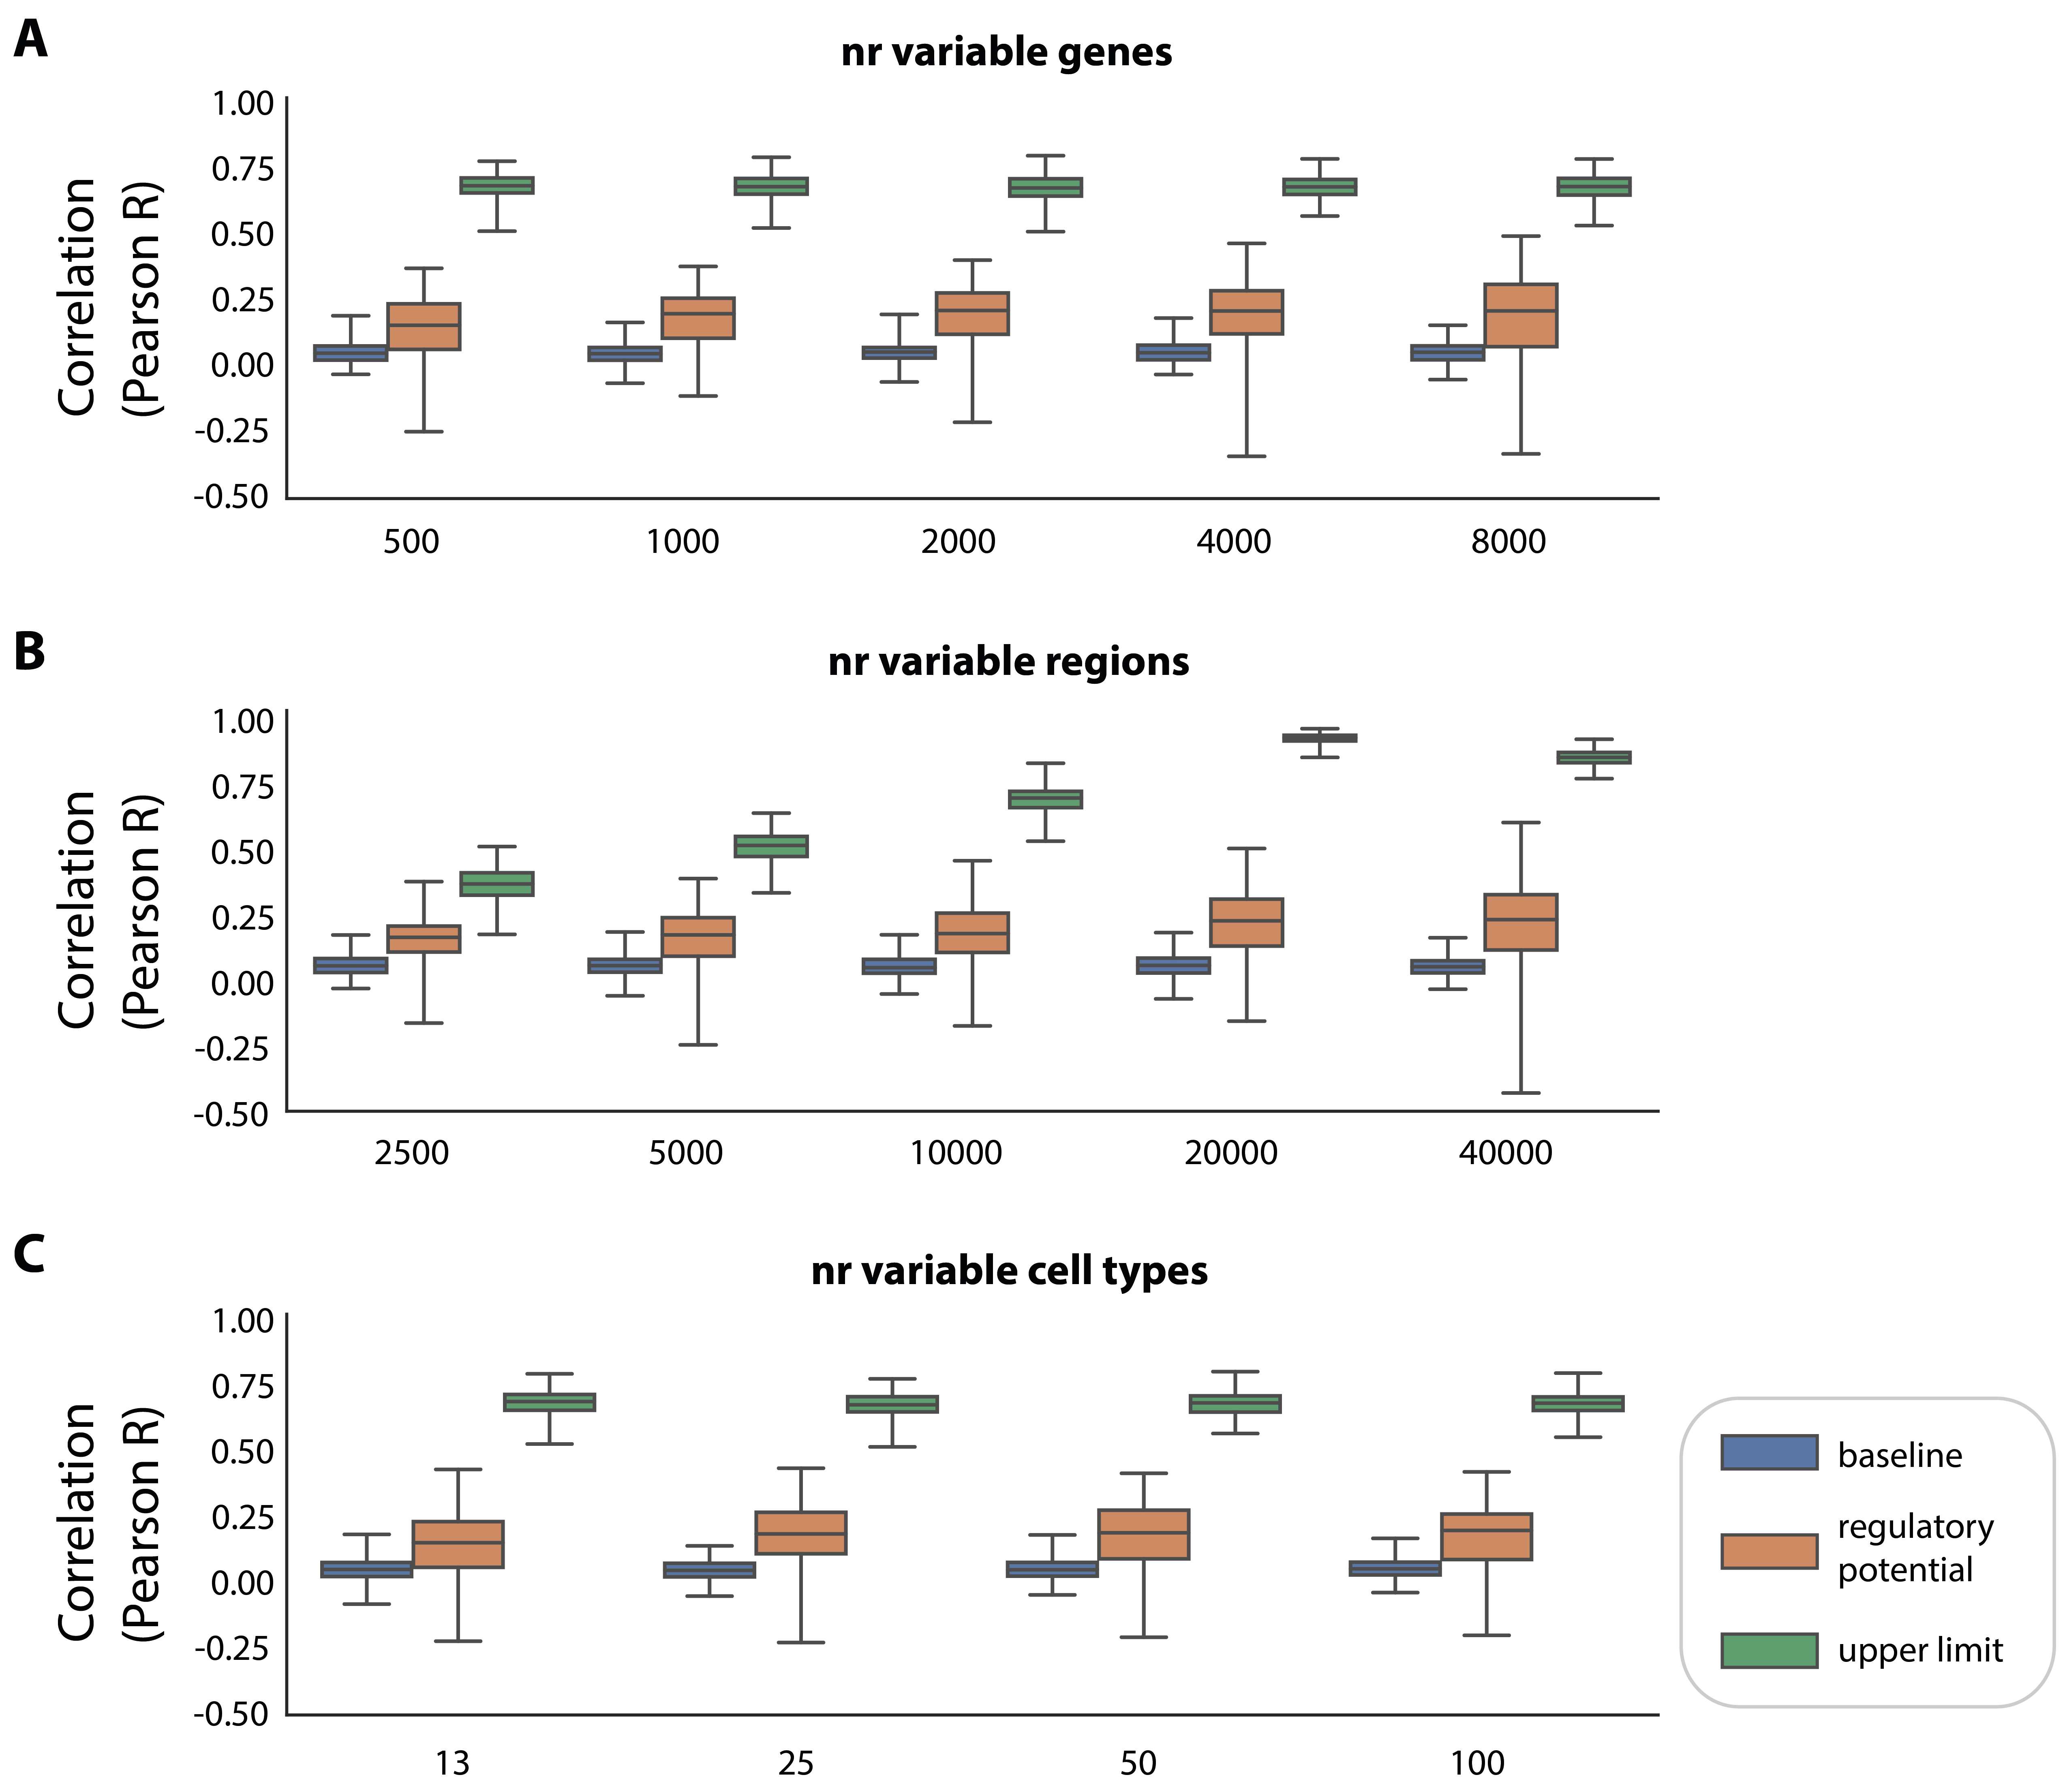
\includegraphics[width=\linewidth]{ch.scepia/imgs/BulkBenchmarks_MvS_Myriad_SuppFig1.png}
    \caption{}
    \label{fig:bulkbenchmark}
\end{figure}
\begin{figure}
    \centering
    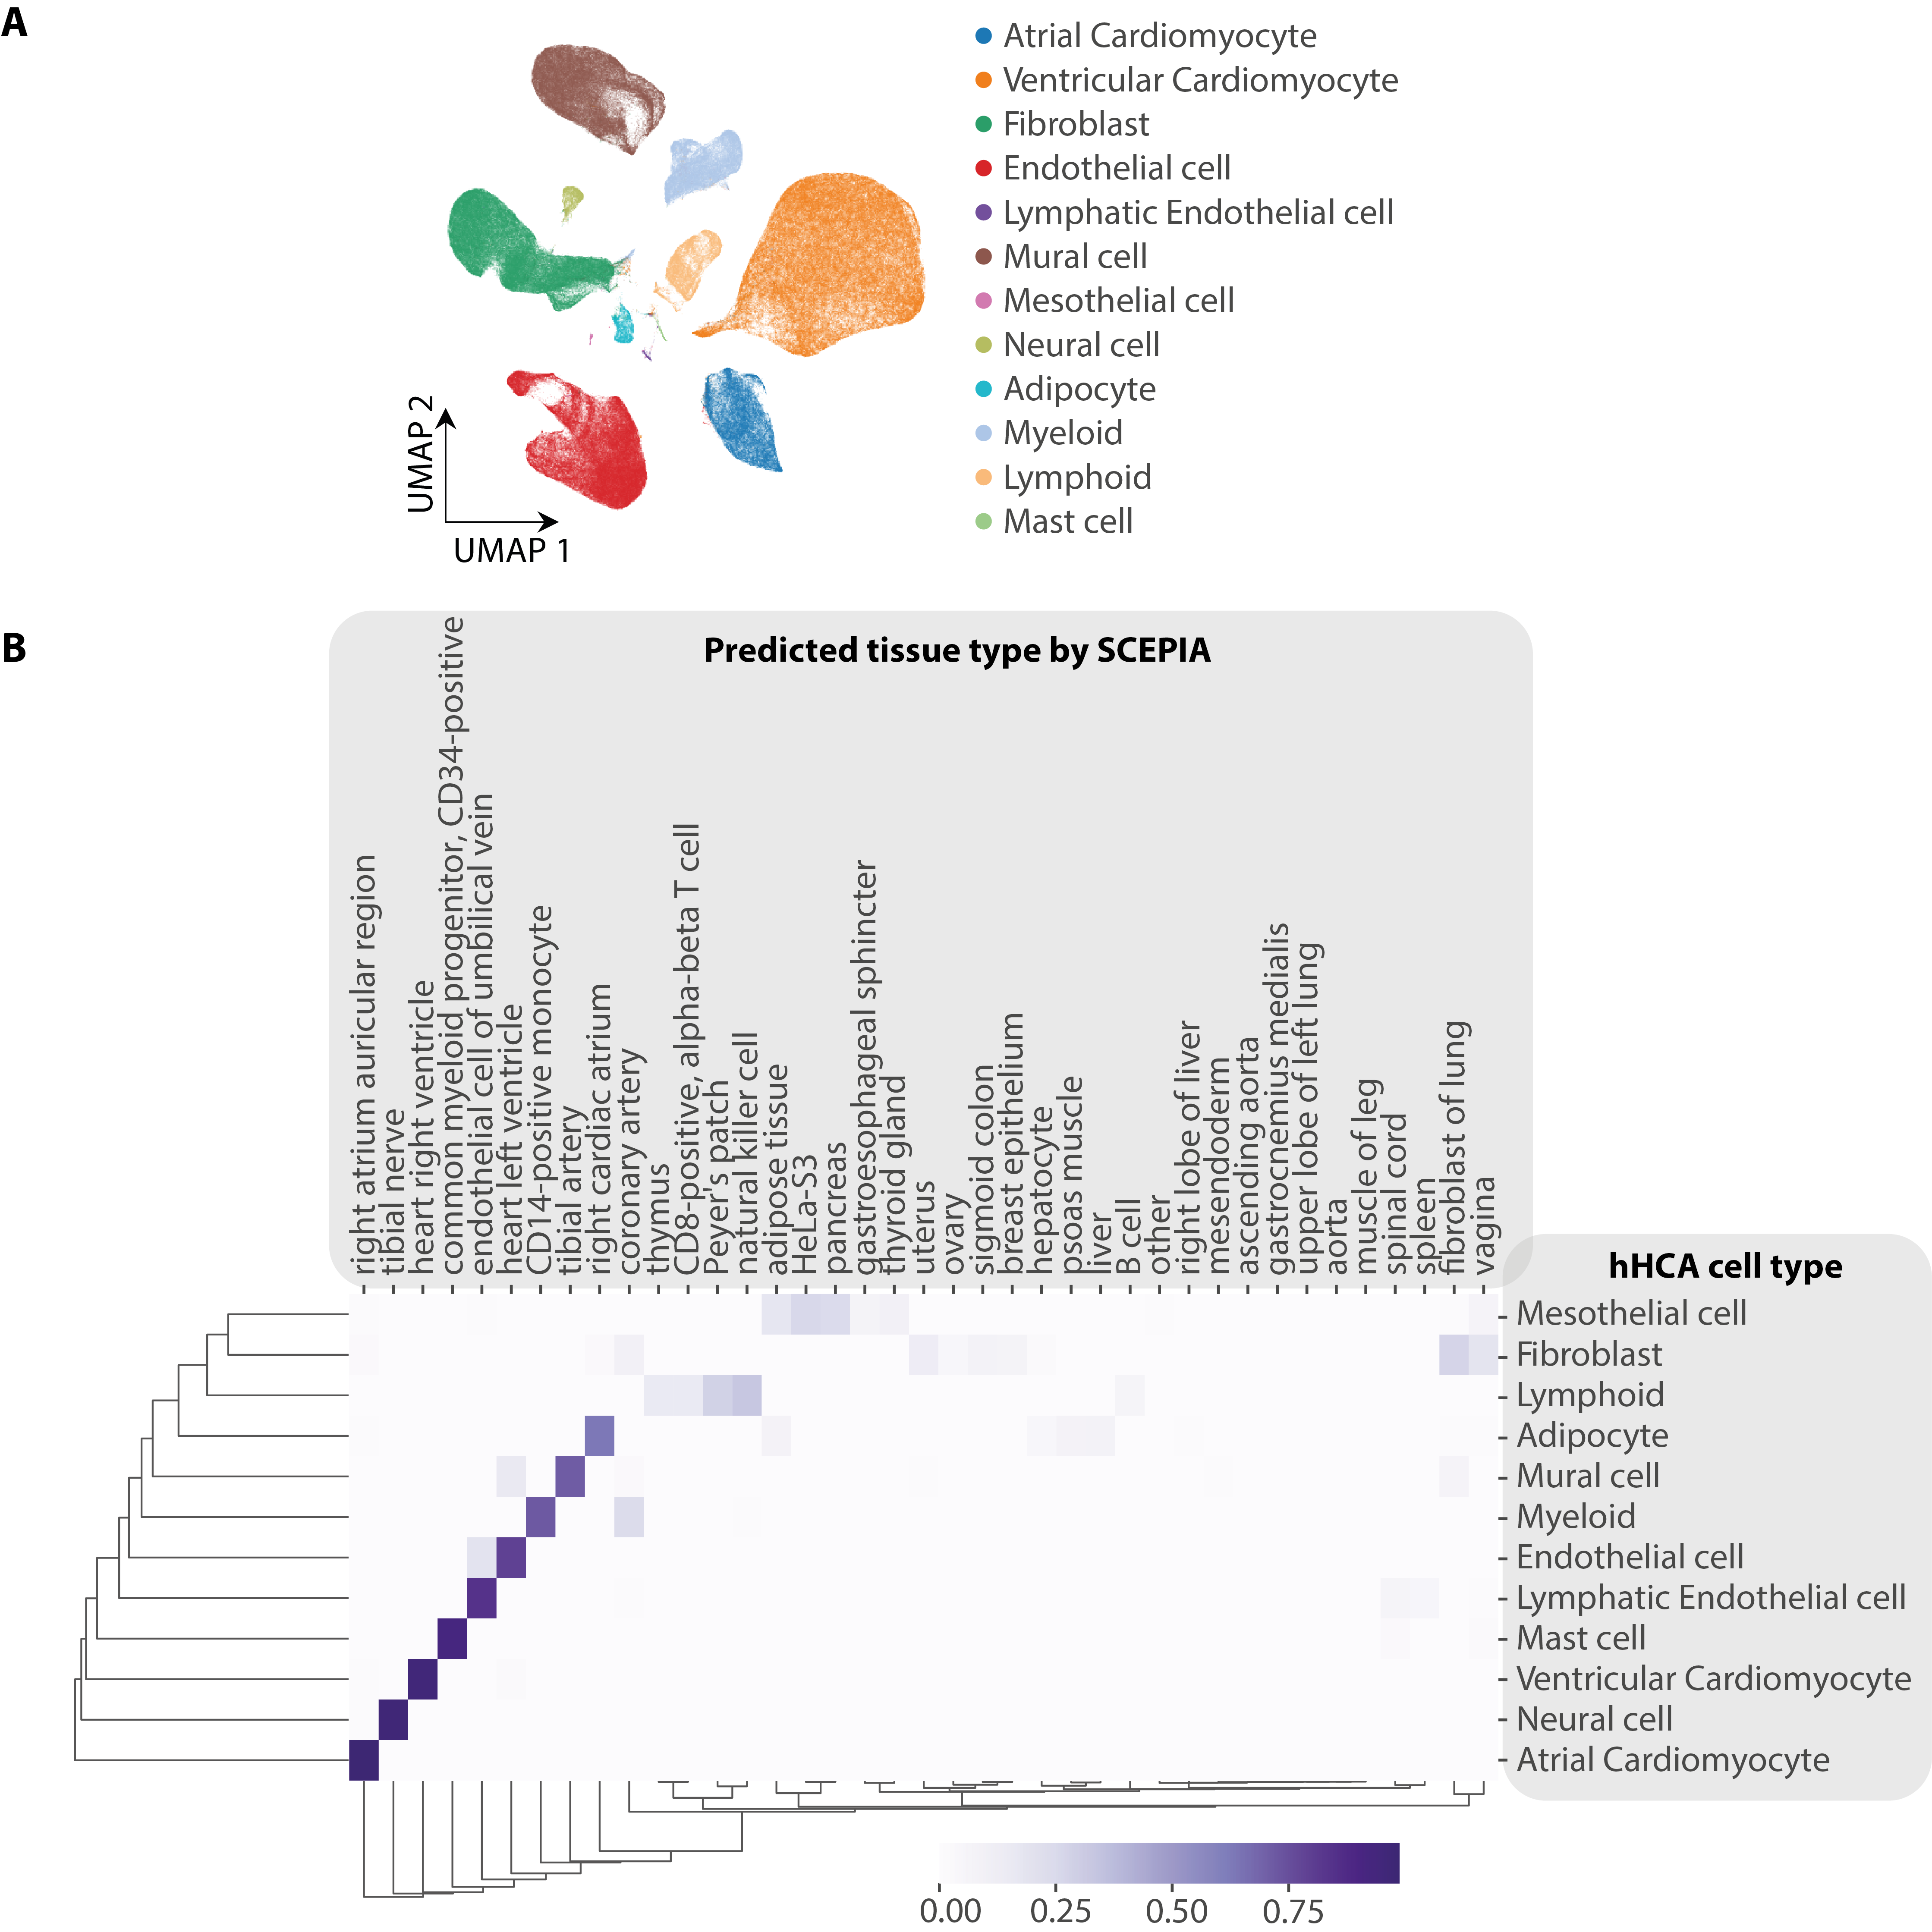
\includegraphics[width=\linewidth]{ch.scepia/imgs/SCEPIA_Annotation_allCells_Myriad_v5_SuppFigAnno.png}
    \caption{Original annotation of cell types (a) SCEPIA annotation of clusters (b) Highest scoring motifs inferred with SCEPIA run on 700K cells (placeholder) }
    \label{fig:scepia_annotation1}
\end{figure}

\begin{figure}
    \centering
    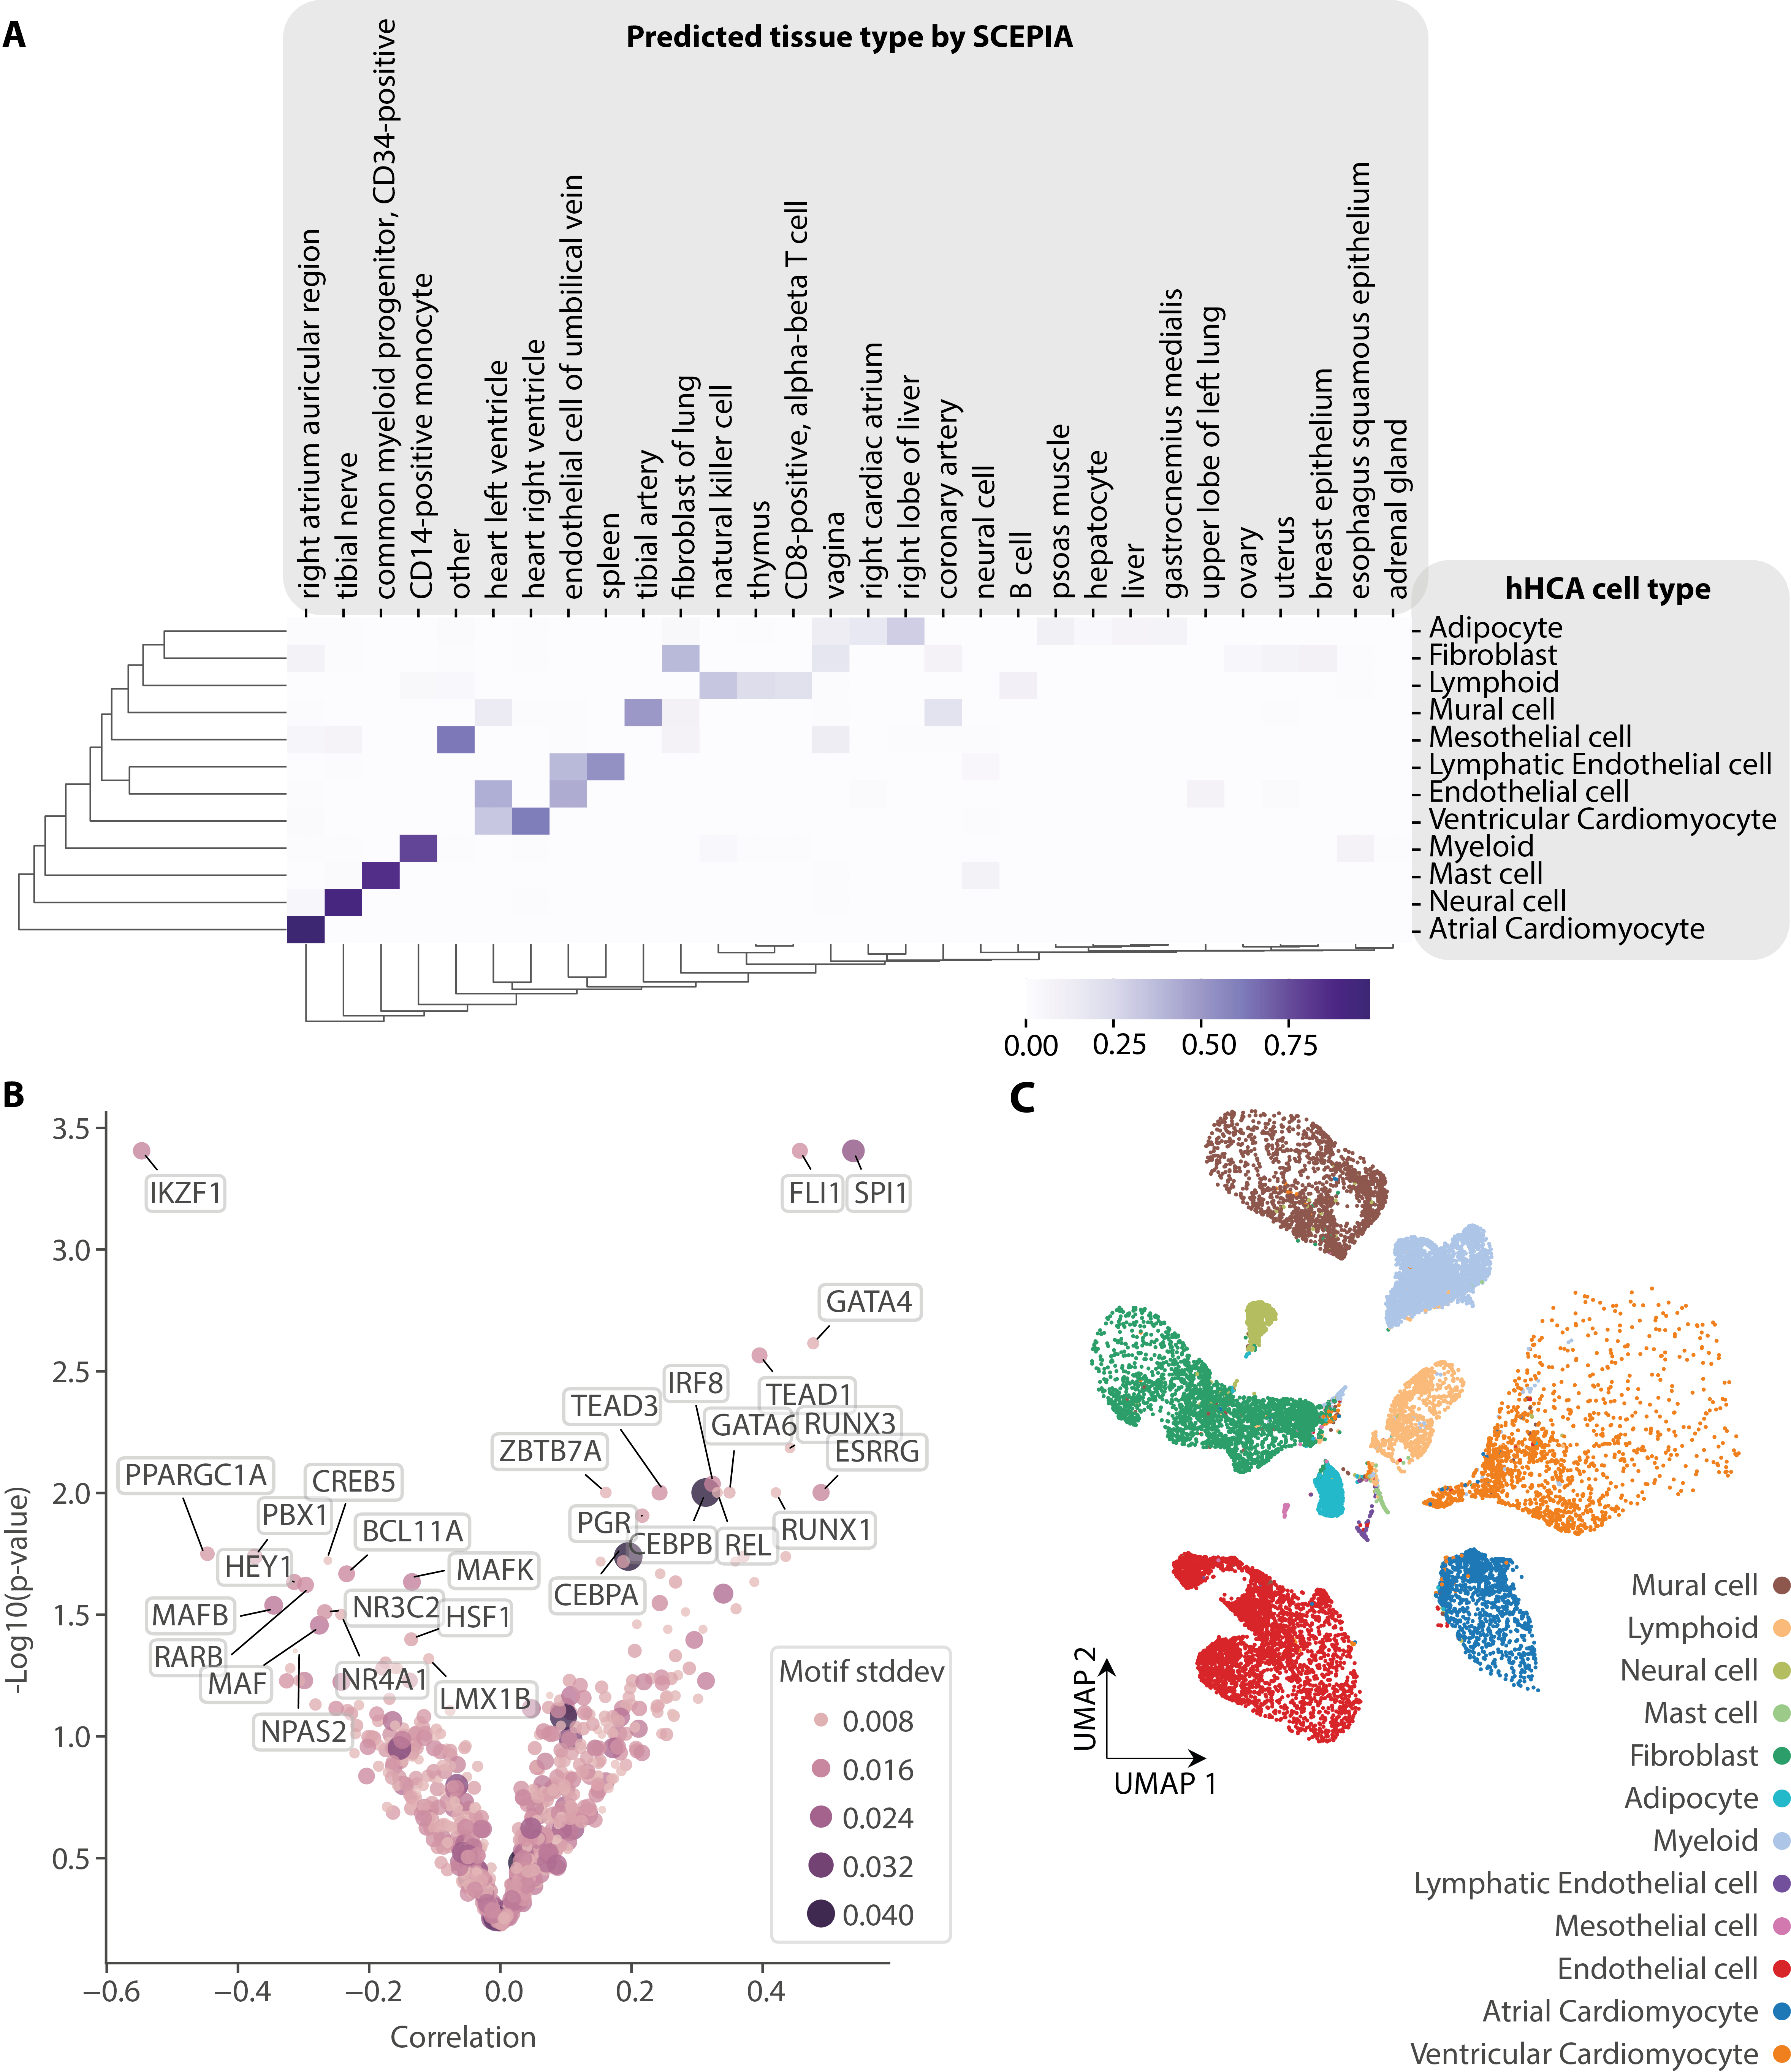
\includegraphics[width=\linewidth]{ch.scepia/imgs/SCEPIAGEOSKETCH_AllCells20000_Myriad_v3_SuppfigGeoAnno.png}
    \caption{SCEPIA run on geosketch of hHCA (A) SCEPIA annotation of clusters (B) Highest scoring motifs inferred with SCEPIA run on 700K cells (C) (placeholder XX) UMAP of 20K geosketch hHCA. }
    \label{fig:geoscepia_results}
\end{figure}

\begin{figure}
    \centering
    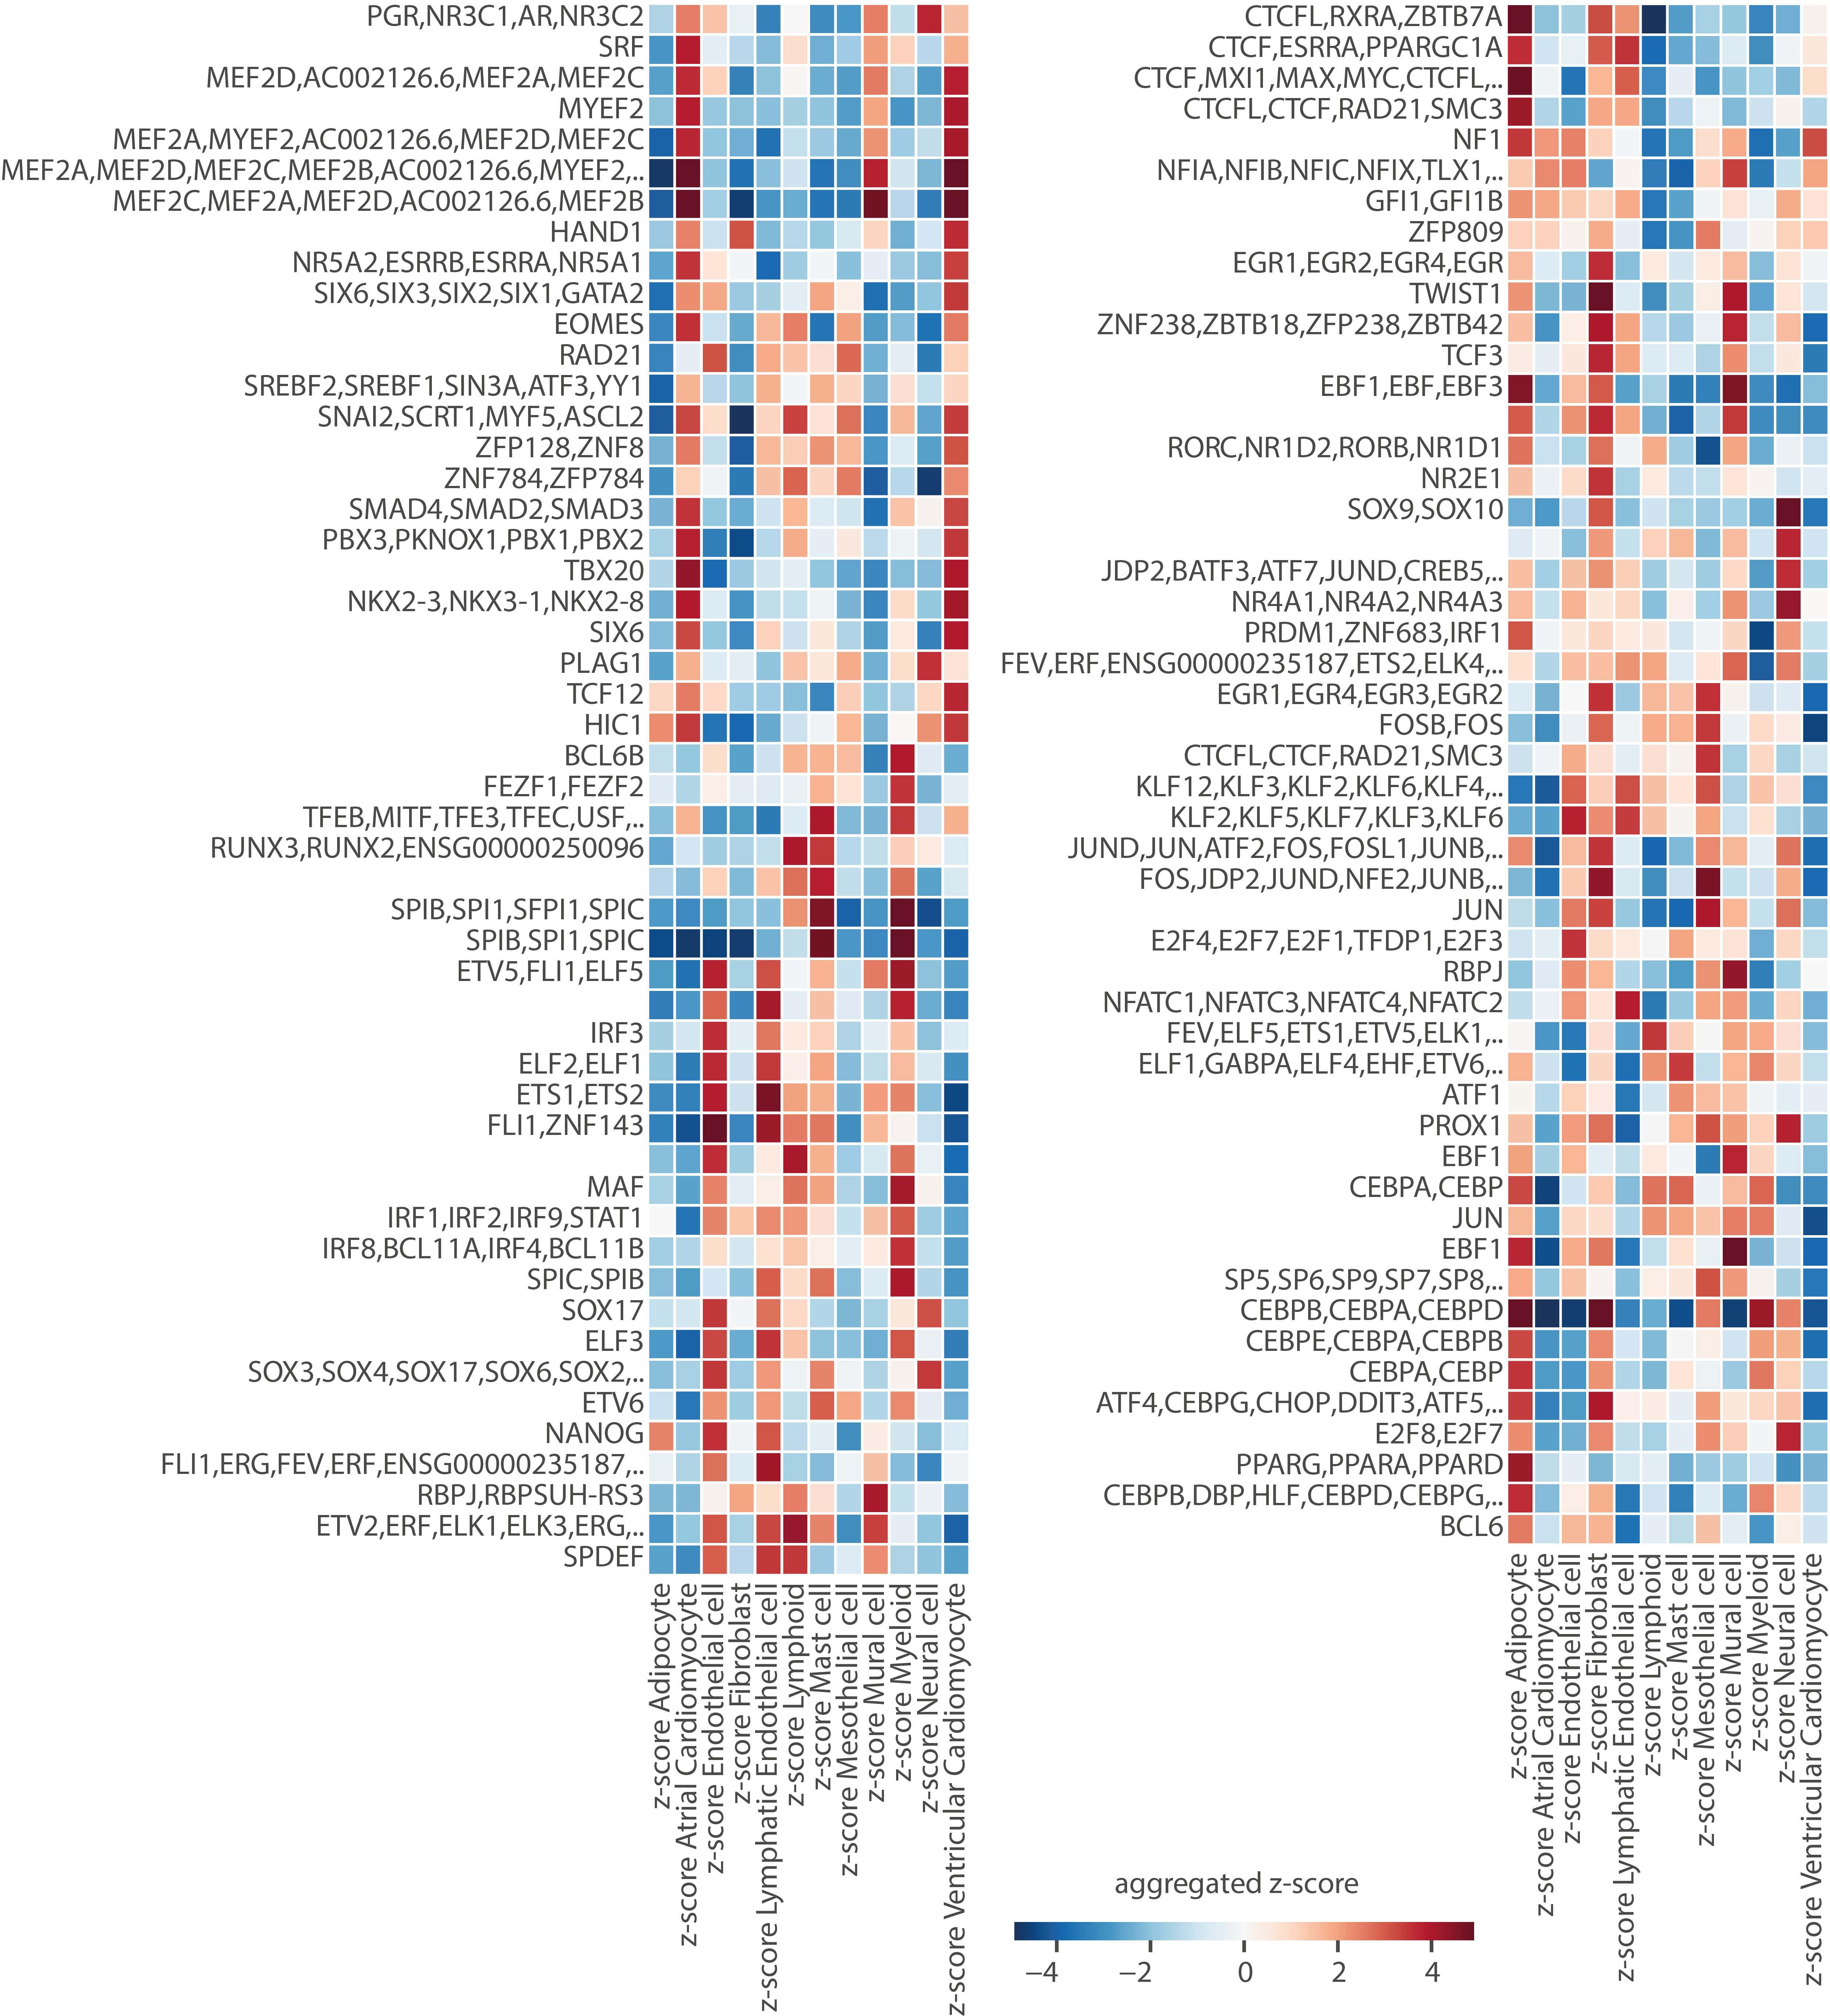
\includegraphics[width=\linewidth]{ch.scepia/imgs/Maelstrom_AllHitsAbove3.5_Myriad_SuppFigMaelstromHM.png}
    \caption{Maelstrom motif analysis output (z-score > 3.5) of the hHCA scATAC-seq cluster averages.}
    \label{fig:scepia_maelstromhm}
\end{figure}

\begin{figure}
    \centering
    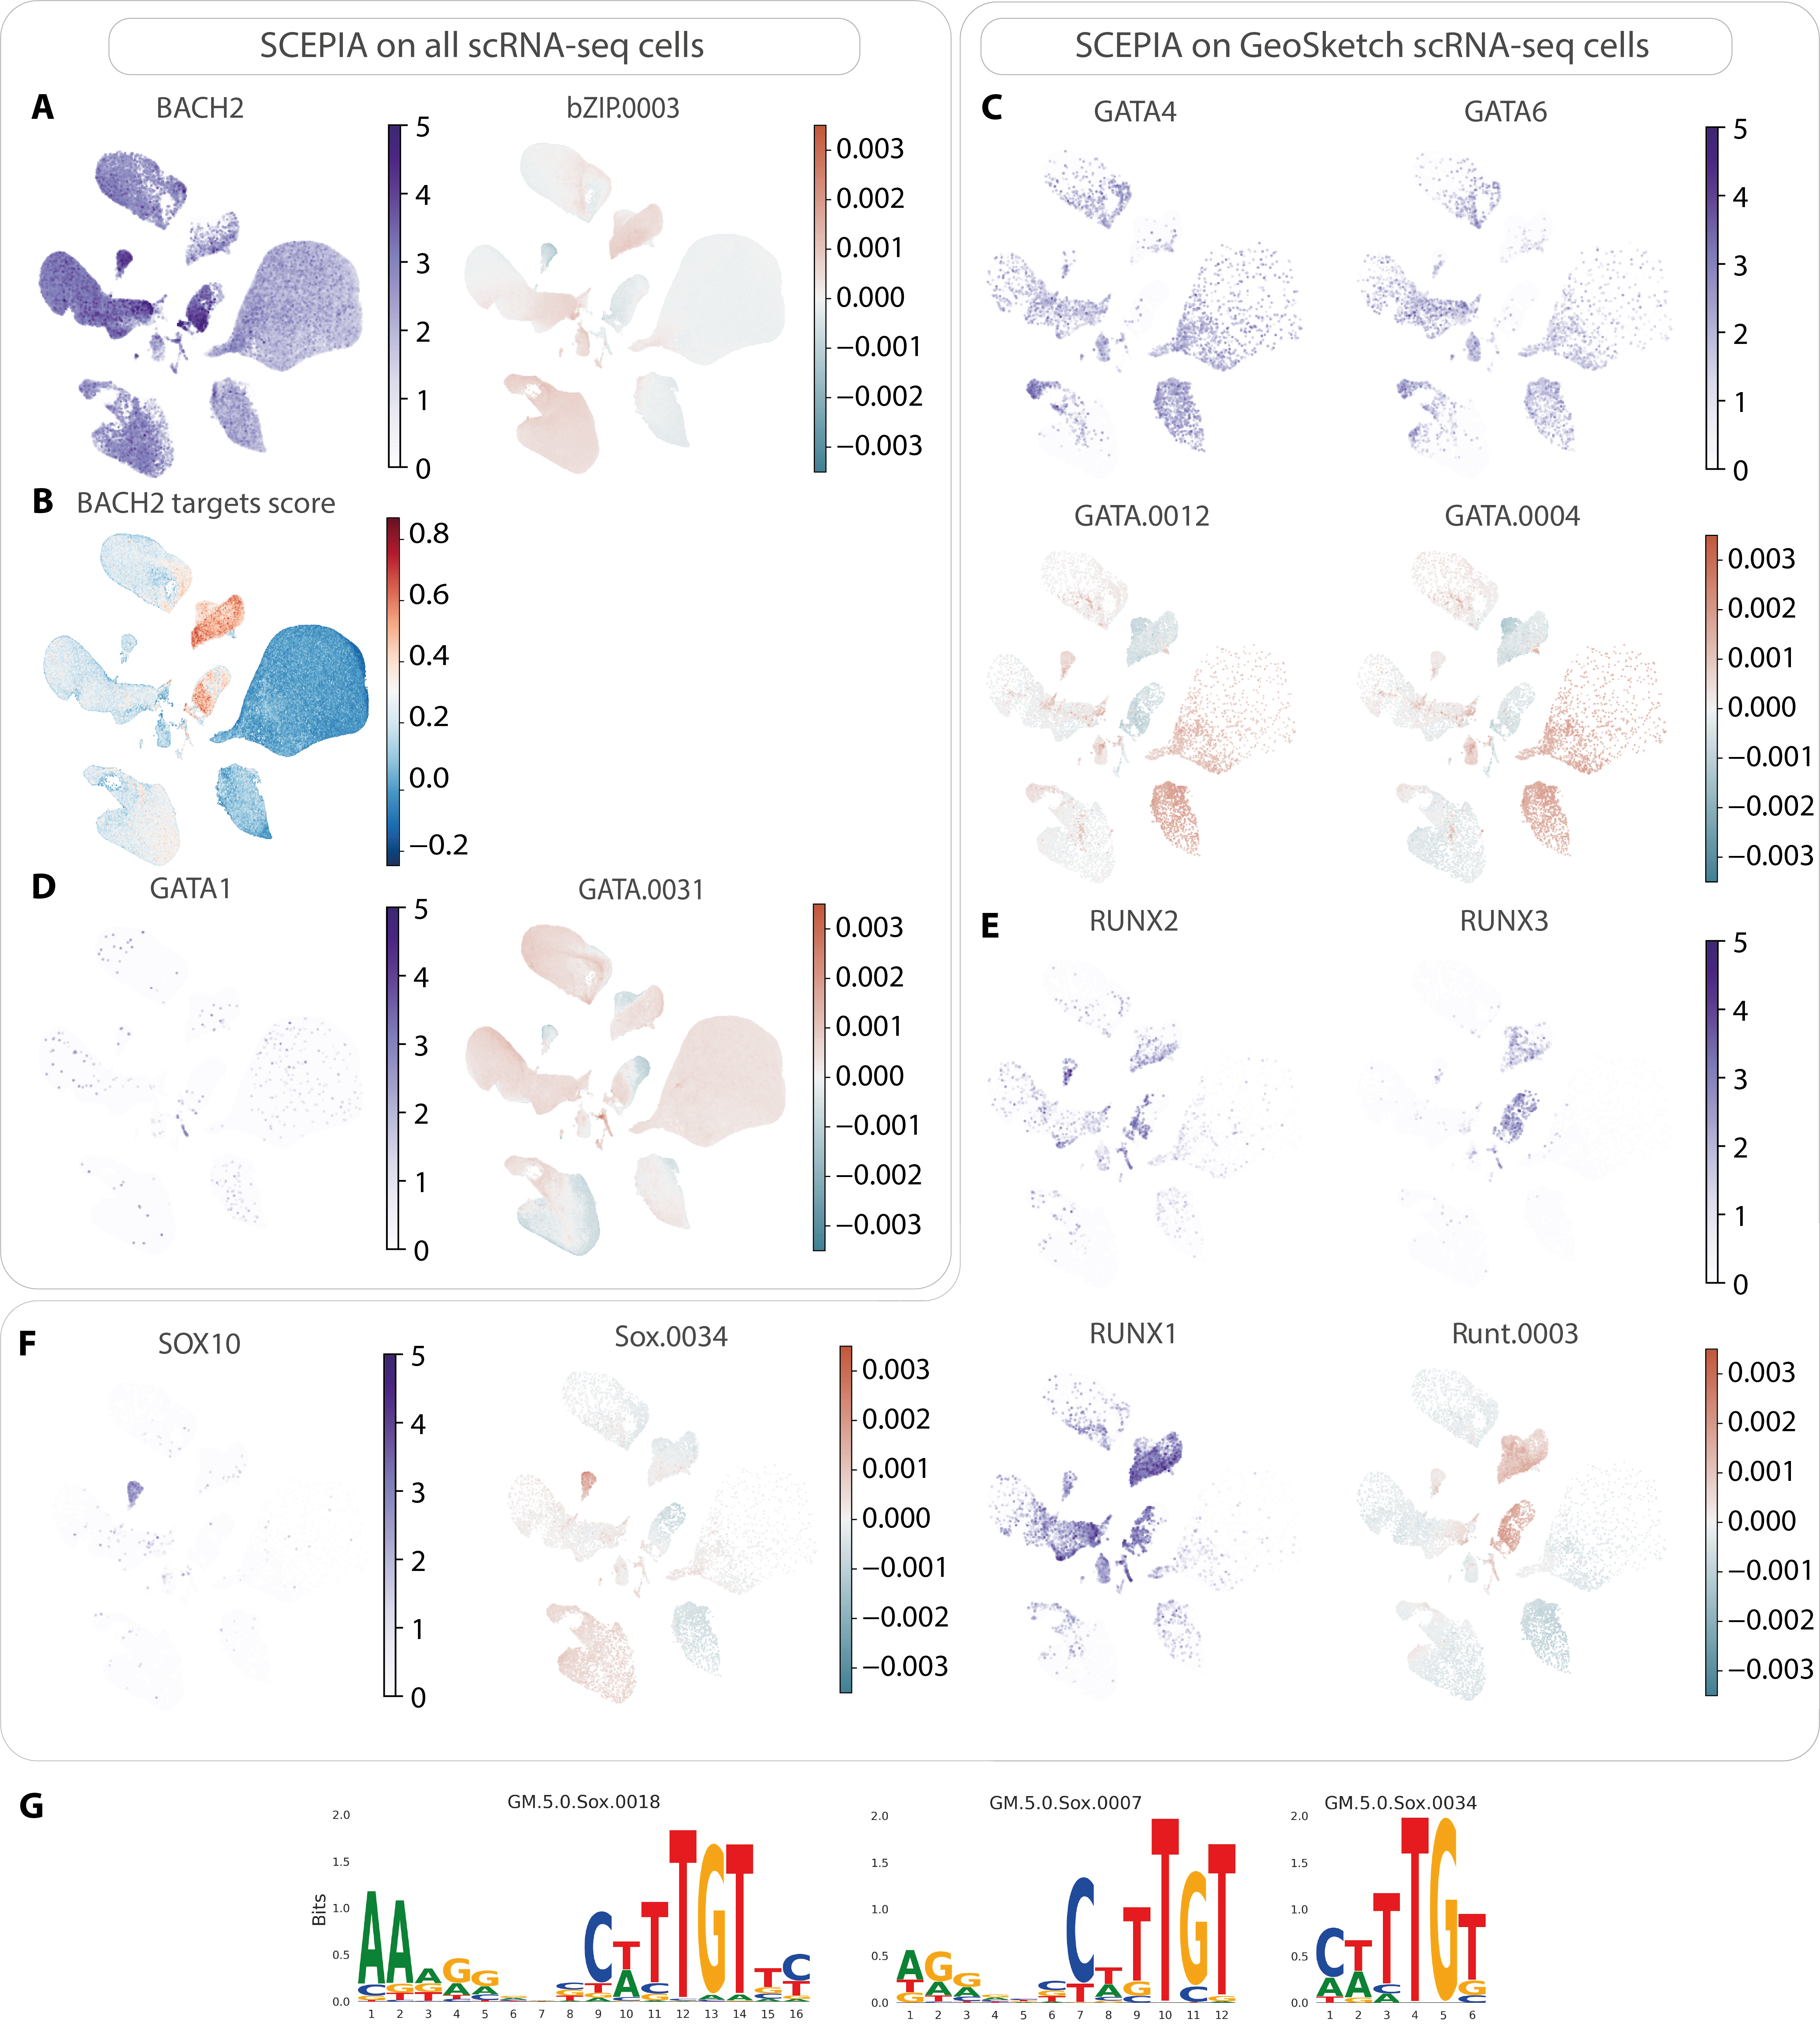
\includegraphics[height=1\linewidth]{ch.scepia/imgs/SCEPIA_SCEPIAGEO_BiologicalExamples_Myriad_v9_SuppFigFeatures1.png}
    \caption{Examples of SCEPIA and geosketch $+$ SCEPIA run \textcolor{red}{(\textbf{B}) Compound expression levels as calculated with scanpy\'s gene_score function, of 57 BACH2 target genes. Target genes taken from ChIP Atlas (REFXX) results for BACH2 ChIPs in differring cell lines and "ChIP score" \> 100.}}
    \label{fig:scepia_features1}
\end{figure}

\begin{figure}
    \centering
    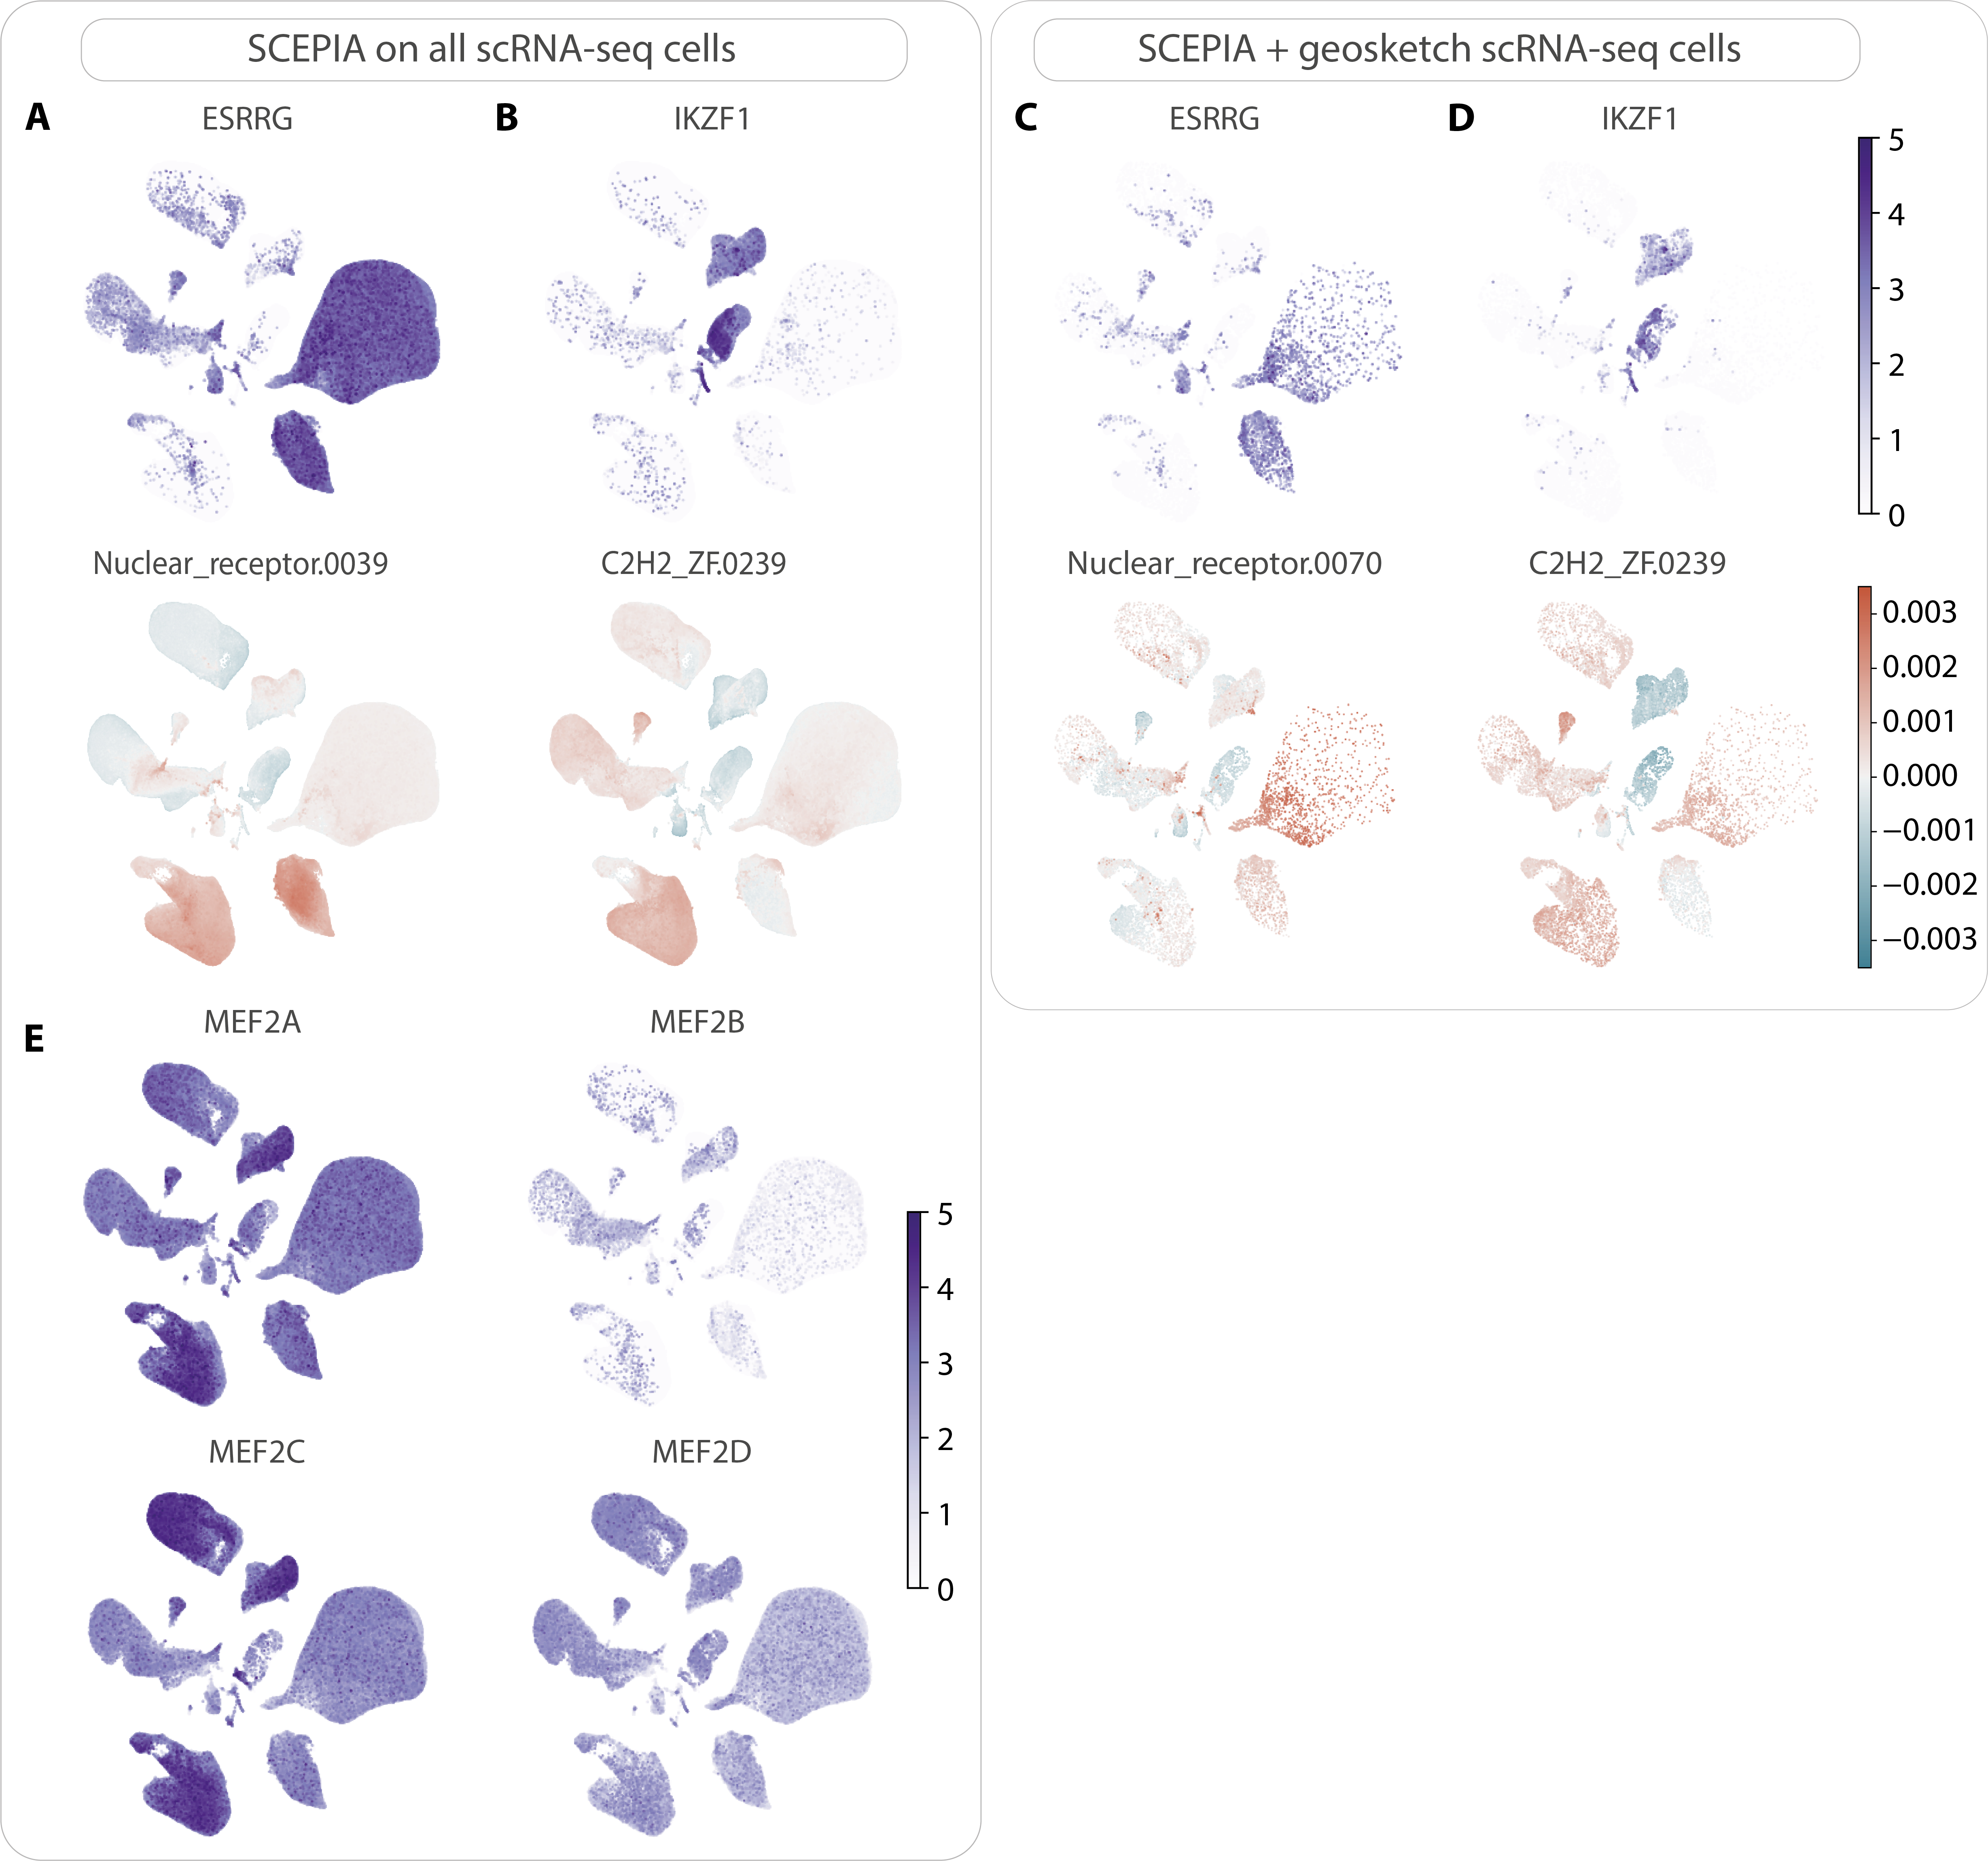
\includegraphics[height=0.666\linewidth]{ch.scepia/imgs/SCEPIA_SCEPIAGEO_BiologicalExamples_Myriad_v4_SuppFigFeatures2.png}
    \caption{Examples of SCEPIA and geosketch $+$ SCEPiA run}
    \label{fig:scepia_features2}
\end{figure}
\begin{table}[htbp]
    \centering
    \caption{\textbf{SCEPIA output for \textit{MEF2}-family factors}. Correlation table output of SCEPIA run on the whole hHCA dataset, selected for the absolute highest correlating motif for each of the \textit{MEF2} factors.}
    \label{tab:corrtable_SCEPIA}
    \begin{tabular}{lcccccc}
        \toprule
        \textbf{Factor} & \textbf{Motif} & \textbf{Correlation} & \textbf{Abs Correlation} & \textbf{P-value} & \textbf{P Adj} & \textbf{Motif Stddev} \\
        \midrule
        MEF2A & GM.5.0.MADS\_box.0007 & 0.3169 & 0.3169 & 0.0076 & 0.0874 & 0.0119 \\
        MEF2C & GM.5.0.MADS\_box.0019 & 0.2123 & 0.2123 & 0.0279 & 0.1446 & 0.0159 \\
        MEF2B & GM.5.0.MADS\_box.0003 & -0.0640 & 0.0640 & 0.1763 & 0.1446 & 0.0177 \\
        MEF2D & GM.5.0.MADS\_box.0002 & -0.0284 & 0.0284 & 0.3082 & 0.4337 & 0.0171 \\
        \bottomrule
    \end{tabular}
\end{table}

\begin{table}[htbp]
    \centering
    \caption{\textbf{SCEPIA output for \textit{MEF2}-family factors}. Correlation table output of SCEPIA + GeoSketch run on the whole hHCA dataset, selected for the absolute highest correlating motif for each of the \textit{MEF2} factors.}
    \label{tab:corrtable_GeoSCEPIA}
    \begin{tabular}{lcccccc}
        \toprule
        \textbf{Factor} & \textbf{Motif} & \textbf{Correlation} & \textbf{Abs Correlation} & \textbf{P-value} & \textbf{P Adj} & \textbf{Motif Stddev} \\
        \midrule
        MEF2C & GM.5.0.MADS\_box.0019 & 0.1503 & 0.1503 & 0.0380 & 0.1612 & 0.0120 \\
        MEF2A & GM.5.0.MADS\_box.0014 & 0.1501 & 0.1501 & 0.0381 & 0.1667 & 0.0144 \\
        MEF2D & GM.5.0.MADS\_box.0014 & 0.1054 & 0.1054 & 0.0756 & 0.1024 & 0.0144 \\
        MEF2B & GM.5.0.MADS\_box.0003 & -0.0663 & 0.0663 & 0.1433 & 0.1591 & 0.0280 \\
        \bottomrule
    \end{tabular}
\end{table}

\begin{table}
    \centering
    \caption{\textbf{The significance of improvements in the single-cell SCEPIA analyses per cell type.} Testing the significance of improvements between Pearson correlations as calculated for the baseline comparison and SCEPIA with Maelstrom, for each of the 7 scRNA-seq subsets and per cell type. The same was also done for the SCEPIA with Maelstrom correlations, with or without the GeoSketch run (right column). P-values were calculated with a one-sided Wilcoxon signed-rank test.}
    \label{tab:significance_scbenchmark}
    \begin{tabular}{llllcc}
        \toprule
         &  Median Baseline&Median SCEPIA&Median SCEPIA + GeoSketch& \textbf{Baseline vs SCEPIA}& \textbf{SCEPIA vs SCEPIA+ GeoSketch}\\
        \midrule
        Atrial Cardiomyocyte  &  0.08&0.27&0.55& 0.0078& 0.0078\\
        Ventricular Cardiomyocyte  &  0.12&0.38&0.54& 0.0078& 0.0078\\
        Fibroblast  &  -0.02&0.34&0.45& 0.0078& 0.1094\\
        Endothelial cell  &  0.12&0.30&0.38& 0.0078& 0.0078\\
        Lymphatic Endothelial cell  &  0.08&0.18&0.34& 0.0547& 0.0156\\
        Mural cell  &  0.08&0.23&0.22& 0.1484& 0.5313\\
        Mesothelial cell  &  0.15&0.14&0.11& 0.5938& 0.8516\\
        Neural cell  &  0.13&0.37&0.31& 0.0078& 0.6563\\
        Adipocyte  &  0.10&0.34&0.34& 0.0156& 0.0781\\
        Myeloid  &  0.26&0.58&0.66& 0.0078& 0.0391\\
        Lymphoid  &  0.00&0.39&0.55& 0.0078& 0.1094\\
        Mast cell  &  0.08&0.45&0.52& 0.0078& 0.1094\\
        \bottomrule
    \end{tabular}
\end{table}